\documentclass[]{article}
\usepackage{lmodern}
\usepackage{amssymb,amsmath}
\usepackage{ifxetex,ifluatex}
\usepackage{fixltx2e} % provides \textsubscript
\ifnum 0\ifxetex 1\fi\ifluatex 1\fi=0 % if pdftex
  \usepackage[T1]{fontenc}
  \usepackage[utf8]{inputenc}
\else % if luatex or xelatex
  \ifxetex
    \usepackage{mathspec}
  \else
    \usepackage{fontspec}
  \fi
  \defaultfontfeatures{Ligatures=TeX,Scale=MatchLowercase}
\fi
% use upquote if available, for straight quotes in verbatim environments
\IfFileExists{upquote.sty}{\usepackage{upquote}}{}
% use microtype if available
\IfFileExists{microtype.sty}{%
\usepackage{microtype}
\UseMicrotypeSet[protrusion]{basicmath} % disable protrusion for tt fonts
}{}
\usepackage[margin=2.54cm]{geometry}
\usepackage{hyperref}
\hypersetup{unicode=true,
            pdftitle={Assignment: Temporal Diversity},
            pdfauthor={Michelle Benavidez; Z620: Quantitative Biodiversity, Indiana University},
            pdfborder={0 0 0},
            breaklinks=true}
\urlstyle{same}  % don't use monospace font for urls
\usepackage{color}
\usepackage{fancyvrb}
\newcommand{\VerbBar}{|}
\newcommand{\VERB}{\Verb[commandchars=\\\{\}]}
\DefineVerbatimEnvironment{Highlighting}{Verbatim}{commandchars=\\\{\}}
% Add ',fontsize=\small' for more characters per line
\usepackage{framed}
\definecolor{shadecolor}{RGB}{248,248,248}
\newenvironment{Shaded}{\begin{snugshade}}{\end{snugshade}}
\newcommand{\KeywordTok}[1]{\textcolor[rgb]{0.13,0.29,0.53}{\textbf{{#1}}}}
\newcommand{\DataTypeTok}[1]{\textcolor[rgb]{0.13,0.29,0.53}{{#1}}}
\newcommand{\DecValTok}[1]{\textcolor[rgb]{0.00,0.00,0.81}{{#1}}}
\newcommand{\BaseNTok}[1]{\textcolor[rgb]{0.00,0.00,0.81}{{#1}}}
\newcommand{\FloatTok}[1]{\textcolor[rgb]{0.00,0.00,0.81}{{#1}}}
\newcommand{\ConstantTok}[1]{\textcolor[rgb]{0.00,0.00,0.00}{{#1}}}
\newcommand{\CharTok}[1]{\textcolor[rgb]{0.31,0.60,0.02}{{#1}}}
\newcommand{\SpecialCharTok}[1]{\textcolor[rgb]{0.00,0.00,0.00}{{#1}}}
\newcommand{\StringTok}[1]{\textcolor[rgb]{0.31,0.60,0.02}{{#1}}}
\newcommand{\VerbatimStringTok}[1]{\textcolor[rgb]{0.31,0.60,0.02}{{#1}}}
\newcommand{\SpecialStringTok}[1]{\textcolor[rgb]{0.31,0.60,0.02}{{#1}}}
\newcommand{\ImportTok}[1]{{#1}}
\newcommand{\CommentTok}[1]{\textcolor[rgb]{0.56,0.35,0.01}{\textit{{#1}}}}
\newcommand{\DocumentationTok}[1]{\textcolor[rgb]{0.56,0.35,0.01}{\textbf{\textit{{#1}}}}}
\newcommand{\AnnotationTok}[1]{\textcolor[rgb]{0.56,0.35,0.01}{\textbf{\textit{{#1}}}}}
\newcommand{\CommentVarTok}[1]{\textcolor[rgb]{0.56,0.35,0.01}{\textbf{\textit{{#1}}}}}
\newcommand{\OtherTok}[1]{\textcolor[rgb]{0.56,0.35,0.01}{{#1}}}
\newcommand{\FunctionTok}[1]{\textcolor[rgb]{0.00,0.00,0.00}{{#1}}}
\newcommand{\VariableTok}[1]{\textcolor[rgb]{0.00,0.00,0.00}{{#1}}}
\newcommand{\ControlFlowTok}[1]{\textcolor[rgb]{0.13,0.29,0.53}{\textbf{{#1}}}}
\newcommand{\OperatorTok}[1]{\textcolor[rgb]{0.81,0.36,0.00}{\textbf{{#1}}}}
\newcommand{\BuiltInTok}[1]{{#1}}
\newcommand{\ExtensionTok}[1]{{#1}}
\newcommand{\PreprocessorTok}[1]{\textcolor[rgb]{0.56,0.35,0.01}{\textit{{#1}}}}
\newcommand{\AttributeTok}[1]{\textcolor[rgb]{0.77,0.63,0.00}{{#1}}}
\newcommand{\RegionMarkerTok}[1]{{#1}}
\newcommand{\InformationTok}[1]{\textcolor[rgb]{0.56,0.35,0.01}{\textbf{\textit{{#1}}}}}
\newcommand{\WarningTok}[1]{\textcolor[rgb]{0.56,0.35,0.01}{\textbf{\textit{{#1}}}}}
\newcommand{\AlertTok}[1]{\textcolor[rgb]{0.94,0.16,0.16}{{#1}}}
\newcommand{\ErrorTok}[1]{\textcolor[rgb]{0.64,0.00,0.00}{\textbf{{#1}}}}
\newcommand{\NormalTok}[1]{{#1}}
\usepackage{longtable,booktabs}
\usepackage{graphicx,grffile}
\makeatletter
\def\maxwidth{\ifdim\Gin@nat@width>\linewidth\linewidth\else\Gin@nat@width\fi}
\def\maxheight{\ifdim\Gin@nat@height>\textheight\textheight\else\Gin@nat@height\fi}
\makeatother
% Scale images if necessary, so that they will not overflow the page
% margins by default, and it is still possible to overwrite the defaults
% using explicit options in \includegraphics[width, height, ...]{}
\setkeys{Gin}{width=\maxwidth,height=\maxheight,keepaspectratio}
\IfFileExists{parskip.sty}{%
\usepackage{parskip}
}{% else
\setlength{\parindent}{0pt}
\setlength{\parskip}{6pt plus 2pt minus 1pt}
}
\setlength{\emergencystretch}{3em}  % prevent overfull lines
\providecommand{\tightlist}{%
  \setlength{\itemsep}{0pt}\setlength{\parskip}{0pt}}
\setcounter{secnumdepth}{0}
% Redefines (sub)paragraphs to behave more like sections
\ifx\paragraph\undefined\else
\let\oldparagraph\paragraph
\renewcommand{\paragraph}[1]{\oldparagraph{#1}\mbox{}}
\fi
\ifx\subparagraph\undefined\else
\let\oldsubparagraph\subparagraph
\renewcommand{\subparagraph}[1]{\oldsubparagraph{#1}\mbox{}}
\fi

%%% Use protect on footnotes to avoid problems with footnotes in titles
\let\rmarkdownfootnote\footnote%
\def\footnote{\protect\rmarkdownfootnote}

%%% Change title format to be more compact
\usepackage{titling}

% Create subtitle command for use in maketitle
\newcommand{\subtitle}[1]{
  \posttitle{
    \begin{center}\large#1\end{center}
    }
}

\setlength{\droptitle}{-2em}
  \title{Assignment: Temporal Diversity}
  \pretitle{\vspace{\droptitle}\centering\huge}
  \posttitle{\par}
  \author{Michelle Benavidez; Z620: Quantitative Biodiversity, Indiana University}
  \preauthor{\centering\large\emph}
  \postauthor{\par}
  \predate{\centering\large\emph}
  \postdate{\par}
  \date{15 February, 2017}


\begin{document}
\maketitle

\subsection{OVERVIEW}\label{overview}

In this Assignment, we extend our understanding of diversity from the
spatial dimension to the temporal dimension.

After completing this exercise you will know how to:

\begin{enumerate}
\def\labelenumi{\arabic{enumi}.}
\tightlist
\item
  wrangle a large dataset to visualize and analyze time series data
\item
  test hypotheses from experiments with temporal data
\item
  quantify temporal \(\beta\)-diversity and stability
\end{enumerate}

\subsection{Directions:}\label{directions}

\begin{enumerate}
\def\labelenumi{\arabic{enumi}.}
\tightlist
\item
  Change ``Student Name'' on line 3 (above) with your name.
\item
  Complete as much of the exercise as possible during class; what you do
  not complete in class will need to be done on your own outside of
  class.
\item
  Use the Handout as a guide; it contains a more complete description of
  data sets along with the proper scripting needed to carry out the
  exercise.
\item
  Be sure to \textbf{answer the questions} in this exercise document;
  they also correspond to the Handout. Space for your answer is provided
  in this document and indicated by the ``\textgreater{}'' character. If
  you need a second paragraph be sure to start the first line with
  ``\textgreater{}''.
\item
  Before you leave the classroom, \textbf{push} this file to your GitHub
  repo.
\item
  When you are done with the Assignment, \textbf{Knit} the text and code
  into a html file.
\item
  After Knitting, please submit the completed Assignment by creating a
  \textbf{pull request} via GitHub. Your pull request should include
  this file \emph{temporal\_assignment.Rmd} and the html output of
  \texttt{Knitr} (\emph{temporal\_assignment.html}).
\end{enumerate}

\subsection{1) R SETUP}\label{r-setup}

Typically, the first thing you will do in either an R script or an
RMarkdown file is setup your environment. This includes things such as
setting the working directory and loading any packages that you will
need.

In the R code chunk below, provide the code to:

\begin{enumerate}
\def\labelenumi{\arabic{enumi}.}
\tightlist
\item
  clear your R environment,
\item
  print your current working directory,
\item
  set your working directory to your ``\emph{/Week5-Temporal}'' folder,
  and
\item
  load any packages you need to complete the assignment.
\end{enumerate}

\begin{Shaded}
\begin{Highlighting}[]
\KeywordTok{rm}\NormalTok{(}\DataTypeTok{list=}\KeywordTok{ls}\NormalTok{())}
\KeywordTok{getwd}\NormalTok{() }
\end{Highlighting}
\end{Shaded}

\begin{verbatim}
## [1] "C:/Users/Michelle/GitHub/QB2017_Benavidez/Week5-Temporal"
\end{verbatim}

\begin{Shaded}
\begin{Highlighting}[]
\KeywordTok{setwd}\NormalTok{(}\StringTok{"C:/users/Michelle/GitHub/QB2017_Benavidez/Week5-Temporal/"}\NormalTok{)}

\KeywordTok{require}\NormalTok{(vegan)}
\end{Highlighting}
\end{Shaded}

\begin{verbatim}
## Loading required package: vegan
\end{verbatim}

\begin{verbatim}
## Loading required package: permute
\end{verbatim}

\begin{verbatim}
## Loading required package: lattice
\end{verbatim}

\begin{verbatim}
## This is vegan 2.4-2
\end{verbatim}

\begin{Shaded}
\begin{Highlighting}[]
\KeywordTok{require}\NormalTok{(tidyr)}
\end{Highlighting}
\end{Shaded}

\begin{verbatim}
## Loading required package: tidyr
\end{verbatim}

\begin{Shaded}
\begin{Highlighting}[]
\KeywordTok{require}\NormalTok{(dplyr)}
\end{Highlighting}
\end{Shaded}

\begin{verbatim}
## Loading required package: dplyr
\end{verbatim}

\begin{verbatim}
## 
## Attaching package: 'dplyr'
\end{verbatim}

\begin{verbatim}
## The following objects are masked from 'package:stats':
## 
##     filter, lag
\end{verbatim}

\begin{verbatim}
## The following objects are masked from 'package:base':
## 
##     intersect, setdiff, setequal, union
\end{verbatim}

\begin{Shaded}
\begin{Highlighting}[]
\KeywordTok{require}\NormalTok{(codyn)}
\end{Highlighting}
\end{Shaded}

\begin{verbatim}
## Loading required package: codyn
\end{verbatim}

\begin{Shaded}
\begin{Highlighting}[]
\KeywordTok{require}\NormalTok{(ggplot2)}
\end{Highlighting}
\end{Shaded}

\begin{verbatim}
## Loading required package: ggplot2
\end{verbatim}

\begin{Shaded}
\begin{Highlighting}[]
\KeywordTok{require}\NormalTok{(cowplt)}
\end{Highlighting}
\end{Shaded}

\begin{verbatim}
## Loading required package: cowplt
\end{verbatim}

\begin{verbatim}
## Warning in library(package, lib.loc = lib.loc, character.only = TRUE,
## logical.return = TRUE, : there is no package called 'cowplt'
\end{verbatim}

\begin{Shaded}
\begin{Highlighting}[]
\KeywordTok{require}\NormalTok{(MullerPlot)}
\end{Highlighting}
\end{Shaded}

\begin{verbatim}
## Loading required package: MullerPlot
\end{verbatim}

\begin{Shaded}
\begin{Highlighting}[]
\KeywordTok{require}\NormalTok{(RColorBrewer)}
\end{Highlighting}
\end{Shaded}

\begin{verbatim}
## Loading required package: RColorBrewer
\end{verbatim}

\begin{Shaded}
\begin{Highlighting}[]
\KeywordTok{require}\NormalTok{(reshape2)}
\end{Highlighting}
\end{Shaded}

\begin{verbatim}
## Loading required package: reshape2
\end{verbatim}

\begin{verbatim}
## 
## Attaching package: 'reshape2'
\end{verbatim}

\begin{verbatim}
## The following object is masked from 'package:tidyr':
## 
##     smiths
\end{verbatim}

\begin{Shaded}
\begin{Highlighting}[]
\KeywordTok{require}\NormalTok{(lubridate)}
\end{Highlighting}
\end{Shaded}

\begin{verbatim}
## Loading required package: lubridate
\end{verbatim}

\begin{verbatim}
## 
## Attaching package: 'lubridate'
\end{verbatim}

\begin{verbatim}
## The following object is masked from 'package:base':
## 
##     date
\end{verbatim}

\begin{Shaded}
\begin{Highlighting}[]
\KeywordTok{require}\NormalTok{(TTR)}
\end{Highlighting}
\end{Shaded}

\begin{verbatim}
## Loading required package: TTR
\end{verbatim}

\begin{Shaded}
\begin{Highlighting}[]
\KeywordTok{require}\NormalTok{(xtable)}
\end{Highlighting}
\end{Shaded}

\begin{verbatim}
## Loading required package: xtable
\end{verbatim}

\begin{Shaded}
\begin{Highlighting}[]
\KeywordTok{require}\NormalTok{(multcomp)}
\end{Highlighting}
\end{Shaded}

\begin{verbatim}
## Loading required package: multcomp
\end{verbatim}

\begin{verbatim}
## Loading required package: mvtnorm
\end{verbatim}

\begin{verbatim}
## Loading required package: survival
\end{verbatim}

\begin{verbatim}
## Loading required package: TH.data
\end{verbatim}

\begin{verbatim}
## Loading required package: MASS
\end{verbatim}

\begin{verbatim}
## 
## Attaching package: 'MASS'
\end{verbatim}

\begin{verbatim}
## The following object is masked from 'package:dplyr':
## 
##     select
\end{verbatim}

\begin{verbatim}
## 
## Attaching package: 'TH.data'
\end{verbatim}

\begin{verbatim}
## The following object is masked from 'package:MASS':
## 
##     geyser
\end{verbatim}

\begin{Shaded}
\begin{Highlighting}[]
\KeywordTok{require}\NormalTok{(pander)}
\end{Highlighting}
\end{Shaded}

\begin{verbatim}
## Loading required package: pander
\end{verbatim}

\begin{Shaded}
\begin{Highlighting}[]
\KeywordTok{require}\NormalTok{(png)}
\end{Highlighting}
\end{Shaded}

\begin{verbatim}
## Loading required package: png
\end{verbatim}

\begin{Shaded}
\begin{Highlighting}[]
\KeywordTok{require}\NormalTok{(grid)}
\end{Highlighting}
\end{Shaded}

\begin{verbatim}
## Loading required package: grid
\end{verbatim}

\begin{Shaded}
\begin{Highlighting}[]
\KeywordTok{require}\NormalTok{(tseries)}
\end{Highlighting}
\end{Shaded}

\begin{verbatim}
## Loading required package: tseries
\end{verbatim}

\begin{Shaded}
\begin{Highlighting}[]
\KeywordTok{require}\NormalTok{(nlme)}
\end{Highlighting}
\end{Shaded}

\begin{verbatim}
## Loading required package: nlme
\end{verbatim}

\begin{verbatim}
## 
## Attaching package: 'nlme'
\end{verbatim}

\begin{verbatim}
## The following object is masked from 'package:dplyr':
## 
##     collapse
\end{verbatim}

\begin{Shaded}
\begin{Highlighting}[]
\KeywordTok{require}\NormalTok{(forecast)}
\end{Highlighting}
\end{Shaded}

\begin{verbatim}
## Loading required package: forecast
\end{verbatim}

\begin{verbatim}
## Loading required package: zoo
\end{verbatim}

\begin{verbatim}
## 
## Attaching package: 'zoo'
\end{verbatim}

\begin{verbatim}
## The following objects are masked from 'package:base':
## 
##     as.Date, as.Date.numeric
\end{verbatim}

\begin{verbatim}
## Loading required package: timeDate
\end{verbatim}

\begin{verbatim}
## 
## Attaching package: 'timeDate'
\end{verbatim}

\begin{verbatim}
## The following object is masked from 'package:xtable':
## 
##     align
\end{verbatim}

\begin{verbatim}
## This is forecast 7.3
\end{verbatim}

\begin{verbatim}
## 
## Attaching package: 'forecast'
\end{verbatim}

\begin{verbatim}
## The following object is masked from 'package:nlme':
## 
##     getResponse
\end{verbatim}

\begin{Shaded}
\begin{Highlighting}[]
\KeywordTok{require}\NormalTok{(lsmeans)}
\end{Highlighting}
\end{Shaded}

\begin{verbatim}
## Loading required package: lsmeans
\end{verbatim}

\begin{verbatim}
## Loading required package: estimability
\end{verbatim}

\begin{Shaded}
\begin{Highlighting}[]
\KeywordTok{require}\NormalTok{(}\StringTok{"vegan"}\NormalTok{)}
\KeywordTok{require}\NormalTok{(}\StringTok{"ade4"}\NormalTok{)}
\end{Highlighting}
\end{Shaded}

\begin{verbatim}
## Loading required package: ade4
\end{verbatim}

\begin{verbatim}
## 
## Attaching package: 'ade4'
\end{verbatim}

\begin{verbatim}
## The following object is masked from 'package:vegan':
## 
##     cca
\end{verbatim}

\begin{Shaded}
\begin{Highlighting}[]
\KeywordTok{require}\NormalTok{(}\StringTok{"BiodiversityR"}\NormalTok{)}
\end{Highlighting}
\end{Shaded}

\begin{verbatim}
## Loading required package: BiodiversityR
\end{verbatim}

\begin{verbatim}
## Loading required package: tcltk
\end{verbatim}

\begin{verbatim}
## BiodiversityR 2.8-0: Use command BiodiversityRGUI() to launch the Graphical User Interface and to learn about backward compatibility
\end{verbatim}

\begin{Shaded}
\begin{Highlighting}[]
\KeywordTok{require}\NormalTok{(}\StringTok{"gplots"}\NormalTok{)}
\end{Highlighting}
\end{Shaded}

\begin{verbatim}
## Loading required package: gplots
\end{verbatim}

\begin{verbatim}
## 
## Attaching package: 'gplots'
\end{verbatim}

\begin{verbatim}
## The following object is masked from 'package:stats':
## 
##     lowess
\end{verbatim}

\begin{Shaded}
\begin{Highlighting}[]
\KeywordTok{require}\NormalTok{(}\StringTok{"viridis"}\NormalTok{)}
\end{Highlighting}
\end{Shaded}

\begin{verbatim}
## Loading required package: viridis
\end{verbatim}

\begin{Shaded}
\begin{Highlighting}[]
\KeywordTok{require}\NormalTok{(}\StringTok{"indicspecies"}\NormalTok{)}
\end{Highlighting}
\end{Shaded}

\begin{verbatim}
## Loading required package: indicspecies
\end{verbatim}

\subsection{2) LOADING DATA}\label{loading-data}

\subsubsection{Load dataset}\label{load-dataset}

In the R code chunk below, do the following:

\begin{enumerate}
\def\labelenumi{\arabic{enumi}.}
\tightlist
\item
  load the \texttt{portal} dataset from in the ``\emph{/Week5/data}''
  folder, and
\item
  explore the structure of the dataset.
\end{enumerate}

\begin{Shaded}
\begin{Highlighting}[]
\NormalTok{portal <-}\StringTok{ }\KeywordTok{read.table}\NormalTok{(}\StringTok{"data/combined.csv"}\NormalTok{, }\DataTypeTok{sep =} \StringTok{","}\NormalTok{, }\DataTypeTok{header =} \OtherTok{TRUE}\NormalTok{)}
\KeywordTok{summary}\NormalTok{(portal)}
\end{Highlighting}
\end{Shaded}

\begin{verbatim}
##    record_id         month             day            year     
##  Min.   :    1   Min.   : 1.000   Min.   : 1.0   Min.   :1977  
##  1st Qu.: 8964   1st Qu.: 4.000   1st Qu.: 9.0   1st Qu.:1984  
##  Median :17762   Median : 6.000   Median :16.0   Median :1990  
##  Mean   :17804   Mean   : 6.474   Mean   :16.1   Mean   :1990  
##  3rd Qu.:26655   3rd Qu.:10.000   3rd Qu.:23.0   3rd Qu.:1997  
##  Max.   :35548   Max.   :12.000   Max.   :31.0   Max.   :2002  
##                                                                
##     plot_id        species_id    sex       hindfoot_length
##  Min.   : 1.00   DM     :10596    : 1748   Min.   : 2.00  
##  1st Qu.: 5.00   PP     : 3123   F:15690   1st Qu.:21.00  
##  Median :11.00   DO     : 3027   M:17348   Median :32.00  
##  Mean   :11.34   PB     : 2891             Mean   :29.29  
##  3rd Qu.:17.00   RM     : 2609             3rd Qu.:36.00  
##  Max.   :24.00   DS     : 2504             Max.   :70.00  
##                  (Other):10036             NA's   :3348   
##      weight                   genus               species     
##  Min.   :  4.00   Dipodomys      :16167   merriami    :10596  
##  1st Qu.: 20.00   Chaetodipus    : 6029   penicillatus: 3123  
##  Median : 37.00   Onychomys      : 3267   ordii       : 3027  
##  Mean   : 42.67   Reithrodontomys: 2694   baileyi     : 2891  
##  3rd Qu.: 48.00   Peromyscus     : 2234   megalotis   : 2609  
##  Max.   :280.00   Perognathus    : 1629   spectabilis : 2504  
##  NA's   :2503     (Other)        : 2766   (Other)     :10036  
##       taxa                           plot_type    
##  Bird   :  450   Control                  :15611  
##  Rabbit :   75   Long-term Krat Exclosure : 5118  
##  Reptile:   14   Rodent Exclosure         : 4233  
##  Rodent :34247   Short-term Krat Exclosure: 5906  
##                  Spectab exclosure        : 3918  
##                                                   
## 
\end{verbatim}

\begin{Shaded}
\begin{Highlighting}[]
\NormalTok{portal2=portal[!(portal$taxa %in%}\StringTok{ }\KeywordTok{c}\NormalTok{(}\StringTok{"Bird"}\NormalTok{,}\StringTok{"Rabbit"}\NormalTok{,}\StringTok{"Reptile"}\NormalTok{)),]}
\end{Highlighting}
\end{Shaded}

\textbf{\emph{Question 1}}: Describe some of the attributes of the
\texttt{portal} dataset.

\begin{enumerate}
\def\labelenumi{\alph{enumi}.}
\tightlist
\item
  How many plots are in \texttt{portal}?
\item
  How many rodent species are there in the \texttt{portal} dataset?
\end{enumerate}

\begin{quote}
\textbf{\emph{Answer 1a}}: 24 plots are present\\
\textbf{\emph{Answer 1b}}: After discounting lizards, birds, and
rabbits, 29 species of rodents are present - five of these are entered
as `sp' (i.e.~Dipodomys sp.), so there is a possibility there are more.
\end{quote}

\subsection{3) WRANGLING THE PORTAL
DATASET}\label{wrangling-the-portal-dataset}

In the R code chunk below, do the following:

\begin{enumerate}
\def\labelenumi{\arabic{enumi}.}
\tightlist
\item
  Create a site-by-species matrix for any year of your choosing.
\item
  Create a vector of plot\_type for sites in the site-by-species matrix.
\item
  Analyze alpha diversity (e.g., Shannon/Simpson) across the sites for
  that year.
\item
  Create a PCoA ordination of your site-by-species matrix.
\item
  Using the hypothesis testing tools you learned in the beta-diversity
  module, test the hypothesis that species abundances across sites vary
  as a factor of treatment type (i.e., plot\_type).
\end{enumerate}

\begin{Shaded}
\begin{Highlighting}[]
\NormalTok{portal <-}\StringTok{ }\KeywordTok{unite}\NormalTok{(portal, }\DataTypeTok{col =} \NormalTok{date, }\KeywordTok{c}\NormalTok{(year, month, day), }\DataTypeTok{sep =} \StringTok{"-"}\NormalTok{, }\DataTypeTok{remove =} \OtherTok{FALSE}\NormalTok{)}
\NormalTok{portal <-}\StringTok{ }\KeywordTok{unite}\NormalTok{(portal, }\DataTypeTok{col =} \NormalTok{taxon, }\KeywordTok{c}\NormalTok{(genus, species), }\DataTypeTok{sep =} \StringTok{"_"}\NormalTok{, }\DataTypeTok{remove =} \OtherTok{FALSE}\NormalTok{)}

\NormalTok{time.by.species <-}\StringTok{ }\KeywordTok{group_by}\NormalTok{(portal,year,plot_id) %>%}
\StringTok{  }\KeywordTok{count}\NormalTok{(taxon) %>%}\StringTok{ }\KeywordTok{spread}\NormalTok{(}\DataTypeTok{key=}\NormalTok{taxon,}\DataTypeTok{value=}\NormalTok{n,}\DataTypeTok{fill=}\DecValTok{0}\NormalTok{)}

\NormalTok{dplyr::}\KeywordTok{filter}\NormalTok{(time.by.species,year==}\DecValTok{1981}\NormalTok{, plot_id==}\DecValTok{6}\NormalTok{)}
\end{Highlighting}
\end{Shaded}

\begin{verbatim}
## Source: local data frame [1 x 50]
## Groups: year, plot_id [1]
## 
##    year plot_id Ammodramus_savannarum Ammospermophilus_harrisi
##   <int>   <int>                 <dbl>                    <dbl>
## 1  1981       6                     0                        0
## # ... with 46 more variables: Amphispiza_bilineata <dbl>,
## #   Baiomys_taylori <dbl>, Calamospiza_melanocorys <dbl>,
## #   Callipepla_squamata <dbl>, Campylorhynchus_brunneicapillus <dbl>,
## #   Chaetodipus_baileyi <dbl>, Chaetodipus_intermedius <dbl>,
## #   Chaetodipus_penicillatus <dbl>, Chaetodipus_sp. <dbl>,
## #   Cnemidophorus_tigris <dbl>, Cnemidophorus_uniparens <dbl>,
## #   Crotalus_scutalatus <dbl>, Crotalus_viridis <dbl>,
## #   Dipodomys_merriami <dbl>, Dipodomys_ordii <dbl>, Dipodomys_sp. <dbl>,
## #   Dipodomys_spectabilis <dbl>, Lizard_sp. <dbl>, Neotoma_albigula <dbl>,
## #   Onychomys_leucogaster <dbl>, Onychomys_sp. <dbl>,
## #   Onychomys_torridus <dbl>, Perognathus_flavus <dbl>,
## #   Perognathus_hispidus <dbl>, Peromyscus_eremicus <dbl>,
## #   Peromyscus_leucopus <dbl>, Peromyscus_maniculatus <dbl>,
## #   Pipilo_chlorurus <dbl>, Pipilo_fuscus <dbl>, Pipilo_sp. <dbl>,
## #   Pooecetes_gramineus <dbl>, Reithrodontomys_fulvescens <dbl>,
## #   Reithrodontomys_megalotis <dbl>, Reithrodontomys_montanus <dbl>,
## #   Reithrodontomys_sp. <dbl>, Rodent_sp. <dbl>, Sceloporus_clarki <dbl>,
## #   Sceloporus_undulatus <dbl>, Sigmodon_fulviventer <dbl>,
## #   Sigmodon_hispidus <dbl>, Sigmodon_ochrognathus <dbl>,
## #   Sparrow_sp. <dbl>, Spermophilus_spilosoma <dbl>,
## #   Spermophilus_tereticaudus <dbl>, Sylvilagus_audubonii <dbl>,
## #   Zonotrichia_leucophrys <dbl>
\end{verbatim}

\begin{Shaded}
\begin{Highlighting}[]
\NormalTok{dplyr::}\KeywordTok{filter}\NormalTok{(time.by.species,plot_id==}\DecValTok{6}\NormalTok{)}
\end{Highlighting}
\end{Shaded}

\begin{verbatim}
## Source: local data frame [26 x 50]
## Groups: year, plot_id [26]
## 
##     year plot_id Ammodramus_savannarum Ammospermophilus_harrisi
##    <int>   <int>                 <dbl>                    <dbl>
## 1   1977       6                     0                        0
## 2   1978       6                     0                        0
## 3   1979       6                     0                        0
## 4   1980       6                     0                        0
## 5   1981       6                     0                        0
## 6   1982       6                     0                        0
## 7   1983       6                     0                        0
## 8   1984       6                     0                        0
## 9   1985       6                     0                        0
## 10  1986       6                     0                        0
## # ... with 16 more rows, and 46 more variables:
## #   Amphispiza_bilineata <dbl>, Baiomys_taylori <dbl>,
## #   Calamospiza_melanocorys <dbl>, Callipepla_squamata <dbl>,
## #   Campylorhynchus_brunneicapillus <dbl>, Chaetodipus_baileyi <dbl>,
## #   Chaetodipus_intermedius <dbl>, Chaetodipus_penicillatus <dbl>,
## #   Chaetodipus_sp. <dbl>, Cnemidophorus_tigris <dbl>,
## #   Cnemidophorus_uniparens <dbl>, Crotalus_scutalatus <dbl>,
## #   Crotalus_viridis <dbl>, Dipodomys_merriami <dbl>,
## #   Dipodomys_ordii <dbl>, Dipodomys_sp. <dbl>,
## #   Dipodomys_spectabilis <dbl>, Lizard_sp. <dbl>, Neotoma_albigula <dbl>,
## #   Onychomys_leucogaster <dbl>, Onychomys_sp. <dbl>,
## #   Onychomys_torridus <dbl>, Perognathus_flavus <dbl>,
## #   Perognathus_hispidus <dbl>, Peromyscus_eremicus <dbl>,
## #   Peromyscus_leucopus <dbl>, Peromyscus_maniculatus <dbl>,
## #   Pipilo_chlorurus <dbl>, Pipilo_fuscus <dbl>, Pipilo_sp. <dbl>,
## #   Pooecetes_gramineus <dbl>, Reithrodontomys_fulvescens <dbl>,
## #   Reithrodontomys_megalotis <dbl>, Reithrodontomys_montanus <dbl>,
## #   Reithrodontomys_sp. <dbl>, Rodent_sp. <dbl>, Sceloporus_clarki <dbl>,
## #   Sceloporus_undulatus <dbl>, Sigmodon_fulviventer <dbl>,
## #   Sigmodon_hispidus <dbl>, Sigmodon_ochrognathus <dbl>,
## #   Sparrow_sp. <dbl>, Spermophilus_spilosoma <dbl>,
## #   Spermophilus_tereticaudus <dbl>, Sylvilagus_audubonii <dbl>,
## #   Zonotrichia_leucophrys <dbl>
\end{verbatim}

\begin{Shaded}
\begin{Highlighting}[]
\NormalTok{tbs}\FloatTok{.1981} \NormalTok{<-}\StringTok{ }\NormalTok{time.by.species[}\DecValTok{93}\NormalTok{:}\DecValTok{116}\NormalTok{,]}
\NormalTok{tbs.forpcoa=tbs}\FloatTok{.1981}\NormalTok{[,}\DecValTok{3}\NormalTok{:}\DecValTok{29}\NormalTok{]}

\KeywordTok{diversity}\NormalTok{(tbs}\FloatTok{.1981}\NormalTok{,}\StringTok{"simp"}\NormalTok{)}
\end{Highlighting}
\end{Shaded}

\begin{verbatim}
##  [1] 0.075804885 0.085387908 0.026680132 0.064891372 0.078779145
##  [6] 0.075659866 0.008015427 0.069461919 0.087951923 0.023763036
## [11] 0.090615190 0.113074514 0.098270513 0.098201176 0.046662477
## [16] 0.018845000 0.089932403 0.084542908 0.047558058 0.089832262
## [21] 0.040018256 0.081012731 0.032364314 0.090665212
\end{verbatim}

\begin{Shaded}
\begin{Highlighting}[]
\NormalTok{tbs1981.db=}\KeywordTok{vegdist}\NormalTok{(tbs.forpcoa,}\DataTypeTok{method=}\StringTok{"bray"}\NormalTok{)}

\NormalTok{rodent.pcoa=}\KeywordTok{cmdscale}\NormalTok{(tbs1981.db,}\DataTypeTok{eig=}\NormalTok{T, }\DataTypeTok{k=}\DecValTok{3}\NormalTok{)}
\NormalTok{explainvar1=}\KeywordTok{round}\NormalTok{(rodent.pcoa$eig[}\DecValTok{1}\NormalTok{] /}\StringTok{ }\KeywordTok{sum}\NormalTok{(rodent.pcoa$eig), }\DecValTok{3}\NormalTok{) *}\StringTok{ }\DecValTok{100}
\NormalTok{explainvar2=}\KeywordTok{round}\NormalTok{(rodent.pcoa$eig[}\DecValTok{2}\NormalTok{] /}\StringTok{ }\KeywordTok{sum}\NormalTok{(rodent.pcoa$eig), }\DecValTok{3}\NormalTok{) *}\StringTok{ }\DecValTok{100}
\NormalTok{explainvar3=}\KeywordTok{round}\NormalTok{(rodent.pcoa$eig[}\DecValTok{3}\NormalTok{] /}\StringTok{ }\KeywordTok{sum}\NormalTok{(rodent.pcoa$eig), }\DecValTok{3}\NormalTok{) *}\StringTok{ }\DecValTok{100}
\NormalTok{sum.eig=}\KeywordTok{sum}\NormalTok{(explainvar1,explainvar2,explainvar3)}

\KeywordTok{par}\NormalTok{(}\DataTypeTok{mar =} \KeywordTok{c}\NormalTok{(}\DecValTok{5}\NormalTok{, }\DecValTok{5}\NormalTok{, }\DecValTok{1}\NormalTok{, }\DecValTok{2}\NormalTok{) +}\StringTok{ }\FloatTok{0.1}\NormalTok{)}
\KeywordTok{plot}\NormalTok{(rodent.pcoa$points[ ,}\DecValTok{1}\NormalTok{], rodent.pcoa$points[ ,}\DecValTok{2}\NormalTok{], }\DataTypeTok{ylim =} \KeywordTok{c}\NormalTok{(-}\FloatTok{0.2}\NormalTok{, }\FloatTok{0.7}\NormalTok{),}
    \DataTypeTok{xlab =} \KeywordTok{paste}\NormalTok{(}\StringTok{"PCoA 1 ("}\NormalTok{, explainvar1, }\StringTok{"%)"}\NormalTok{, }\DataTypeTok{sep =} \StringTok{""}\NormalTok{),}
    \DataTypeTok{ylab =} \KeywordTok{paste}\NormalTok{(}\StringTok{"PCoA 2 ("}\NormalTok{, explainvar2, }\StringTok{"%)"}\NormalTok{, }\DataTypeTok{sep =} \StringTok{""}\NormalTok{),}
    \DataTypeTok{pch =} \DecValTok{16}\NormalTok{, }\DataTypeTok{cex =} \FloatTok{2.0}\NormalTok{, }\DataTypeTok{type =} \StringTok{"n"}\NormalTok{, }\DataTypeTok{cex.lab =} \FloatTok{1.5}\NormalTok{, }\DataTypeTok{cex.axis =} \FloatTok{1.2}\NormalTok{, }\DataTypeTok{axes =} \OtherTok{FALSE}\NormalTok{)}
\KeywordTok{axis}\NormalTok{(}\DataTypeTok{side =} \DecValTok{1}\NormalTok{, }\DataTypeTok{labels =} \NormalTok{T, }\DataTypeTok{lwd.ticks =} \DecValTok{2}\NormalTok{, }\DataTypeTok{cex.axis =} \FloatTok{1.2}\NormalTok{, }\DataTypeTok{las =} \DecValTok{1}\NormalTok{) }
\KeywordTok{axis}\NormalTok{(}\DataTypeTok{side =} \DecValTok{2}\NormalTok{, }\DataTypeTok{labels =} \NormalTok{T, }\DataTypeTok{lwd.ticks =} \DecValTok{2}\NormalTok{, }\DataTypeTok{cex.axis =} \FloatTok{1.2}\NormalTok{, }\DataTypeTok{las =} \DecValTok{1}\NormalTok{) }
\KeywordTok{abline}\NormalTok{(}\DataTypeTok{h =} \DecValTok{0}\NormalTok{, }\DataTypeTok{v =} \DecValTok{0}\NormalTok{, }\DataTypeTok{lty =} \DecValTok{3}\NormalTok{)}
\KeywordTok{box}\NormalTok{(}\DataTypeTok{lwd =} \DecValTok{2}\NormalTok{)}
\KeywordTok{points}\NormalTok{(rodent.pcoa$points[ ,}\DecValTok{1}\NormalTok{], rodent.pcoa$points[ ,}\DecValTok{2}\NormalTok{], }
       \DataTypeTok{pch =} \DecValTok{19}\NormalTok{, }\DataTypeTok{cex =} \DecValTok{3}\NormalTok{, }\DataTypeTok{bg =} \StringTok{"gray"}\NormalTok{, }\DataTypeTok{col =} \StringTok{"gray"}\NormalTok{)}
\KeywordTok{text}\NormalTok{(rodent.pcoa$points[ ,}\DecValTok{1}\NormalTok{], rodent.pcoa$points[ ,}\DecValTok{2}\NormalTok{], }
     \DataTypeTok{labels =} \KeywordTok{row.names}\NormalTok{(rodent.pcoa$points))}
\end{Highlighting}
\end{Shaded}

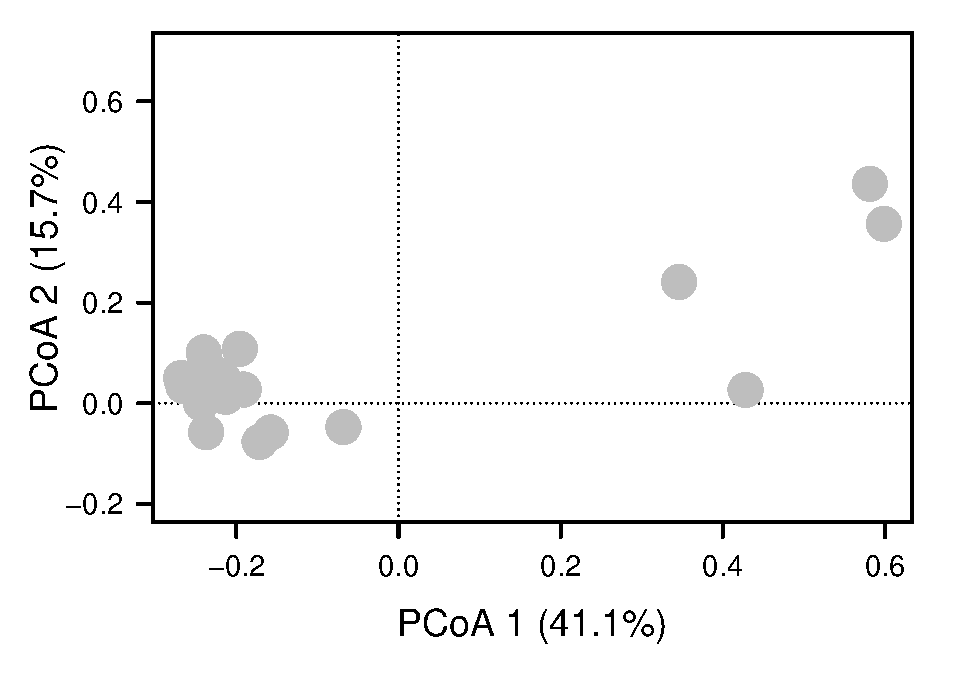
\includegraphics{temporal_assignment_files/figure-latex/unnamed-chunk-3-1.pdf}

\begin{Shaded}
\begin{Highlighting}[]
\NormalTok{rodentREL=tbs.forpcoa}

  \NormalTok{for(i in }\DecValTok{1}\NormalTok{:}\KeywordTok{nrow}\NormalTok{(tbs.forpcoa))\{}
    \NormalTok{rodentREL[i, ] =}\StringTok{ }\NormalTok{tbs.forpcoa[i, ] /}\StringTok{ }\KeywordTok{sum}\NormalTok{(tbs.forpcoa[i, ]) }
  \NormalTok{\}}

\NormalTok{plot=}\KeywordTok{c}\NormalTok{(}\DecValTok{1}\NormalTok{:}\DecValTok{24}\NormalTok{)}
\NormalTok{tbs.stat=tbs}\FloatTok{.1981}\NormalTok{[}\DecValTok{2}\NormalTok{:}\DecValTok{31}\NormalTok{]}
\KeywordTok{adonis}\NormalTok{(tbs.stat~plot,}\DataTypeTok{method=}\StringTok{"bray"}\NormalTok{,}\DataTypeTok{permtations=}\DecValTok{999}\NormalTok{)}
\end{Highlighting}
\end{Shaded}

\begin{verbatim}
## 
## Call:
## adonis(formula = tbs.stat ~ plot, method = "bray", permtations = 999) 
## 
## Permutation: free
## Number of permutations: 999
## 
## Terms added sequentially (first to last)
## 
##           Df SumsOfSqs MeanSqs F.Model      R2 Pr(>F)   
## plot       1    0.7414 0.74137   4.709 0.17631  0.003 **
## Residuals 22    3.4636 0.15744         0.82369          
## Total     23    4.2050                 1.00000          
## ---
## Signif. codes:  0 '***' 0.001 '**' 0.01 '*' 0.05 '.' 0.1 ' ' 1
\end{verbatim}

\textbf{\emph{Question 2}}: Describe how different biodiversity
estimates vary among sites.

\begin{enumerate}
\def\labelenumi{\alph{enumi}.}
\tightlist
\item
  Does diversity vary among sites? Does this correspond to treatment
  type?
\item
  Is treatment type a significant predictor of site dissimilarity?
\end{enumerate}

\begin{quote}
\textbf{\emph{Answer 2a}}: Diversity does vary among sites and this
corresponds to treatment ype. \textbf{\emph{Answer 2b}}: Treatment type
of a significant predictor of site dissimilarity
\end{quote}

\subsection{4) TIME SERIES ANALYSIS}\label{time-series-analysis}

In the R code chunk below, do the following:

\begin{enumerate}
\def\labelenumi{\arabic{enumi}.}
\tightlist
\item
  Create a time-by-species matrix that includes year, month, and
  plot\_id for a site other than plot\_id 2.
\item
  Examine per-hectare rodent abundance using simple moving average
  smoothing.
\item
  Test whether your data meets the assumption of stationarity.
\item
  If it does not meet this asumption, explore wasy to make your data
  stationary.
\item
  Examine and plot time lags using the partial autocorrelation function
  (PACF) and autocorrelation function (ACR).
\item
  Use the tools outlined in the Handout to create an ARMA model.
\end{enumerate}

\begin{Shaded}
\begin{Highlighting}[]
\NormalTok{time.by.spec}\FloatTok{.2} \NormalTok{<-}\StringTok{ }\KeywordTok{filter}\NormalTok{(portal, taxa==}\StringTok{"Rodent"}\NormalTok{) %>%}
\StringTok{  }\KeywordTok{group_by}\NormalTok{(year,month, plot_id) %>%}
\StringTok{  }\KeywordTok{count}\NormalTok{(taxon)}

\NormalTok{time.by.spec}\FloatTok{.2}\NormalTok{$season <-}\StringTok{ }\OtherTok{NA}
\NormalTok{time.by.spec}\FloatTok{.2}\NormalTok{$season <-}\StringTok{ }\NormalTok{time.by.spec}\FloatTok{.2}\NormalTok{$month %in%}\StringTok{ }\KeywordTok{c}\NormalTok{(}\DecValTok{6}\NormalTok{:}\DecValTok{10}\NormalTok{)}

\NormalTok{time.by.spec}\FloatTok{.2}\NormalTok{$season <-}\StringTok{ }\KeywordTok{ifelse}\NormalTok{(time.by.spec}\FloatTok{.2}\NormalTok{$season ==}\StringTok{ }\OtherTok{TRUE}\NormalTok{, }\StringTok{"rain"}\NormalTok{, }\StringTok{"norain"}\NormalTok{)}

\KeywordTok{group_by}\NormalTok{(time.by.spec}\FloatTok{.2}\NormalTok{, year, season)}
\end{Highlighting}
\end{Shaded}

\begin{verbatim}
## Source: local data frame [16,391 x 6]
## Groups: year, season [52]
## 
##     year month plot_id                    taxon     n season
##    <int> <int>   <int>                    <chr> <int>  <chr>
## 1   1977     7       1       Dipodomys_merriami     2   rain
## 2   1977     7       1       Perognathus_flavus     1   rain
## 3   1977     7       2 Chaetodipus_penicillatus     1   rain
## 4   1977     7       2       Dipodomys_merriami     1   rain
## 5   1977     7       2         Neotoma_albigula     1   rain
## 6   1977     7       2      Peromyscus_eremicus     1   rain
## 7   1977     7       3       Dipodomys_merriami     2   rain
## 8   1977     7       3    Dipodomys_spectabilis     1   rain
## 9   1977     7       3         Neotoma_albigula     1   rain
## 10  1977     7       4       Dipodomys_merriami     1   rain
## # ... with 16,381 more rows
\end{verbatim}

\begin{Shaded}
\begin{Highlighting}[]
\NormalTok{abund <-}\StringTok{ }\KeywordTok{filter}\NormalTok{(time.by.spec}\FloatTok{.2}\NormalTok{, plot_id ==}\StringTok{ }\DecValTok{24}\NormalTok{) %>%}\StringTok{ }
\StringTok{  }\KeywordTok{group_by}\NormalTok{(year, season) %>%}
\StringTok{  }\KeywordTok{count}\NormalTok{(}\DataTypeTok{wt =} \NormalTok{n)}

\NormalTok{abund$nn <-}\StringTok{ }\NormalTok{abund$nn *}\StringTok{ }\DecValTok{4}

\NormalTok{abund.ts <-}\StringTok{ }\KeywordTok{ts}\NormalTok{(abund$nn, }\DataTypeTok{frequency =} \DecValTok{2}\NormalTok{, }\DataTypeTok{start =} \KeywordTok{c}\NormalTok{(}\DecValTok{1977}\NormalTok{, }\DecValTok{2}\NormalTok{))}

\KeywordTok{plot.ts}\NormalTok{(abund.ts, }\DataTypeTok{type =} \StringTok{"l"}\NormalTok{, }\DataTypeTok{ylab =} \StringTok{"Rodent Abundance(#/hectare)"}\NormalTok{,}
        \DataTypeTok{xlab =} \StringTok{"Time (year)"}\NormalTok{, }\DataTypeTok{las =} \DecValTok{1}\NormalTok{, }\DataTypeTok{ylim =} \KeywordTok{c}\NormalTok{(}\DecValTok{0}\NormalTok{, }\DecValTok{500}\NormalTok{))}
\end{Highlighting}
\end{Shaded}

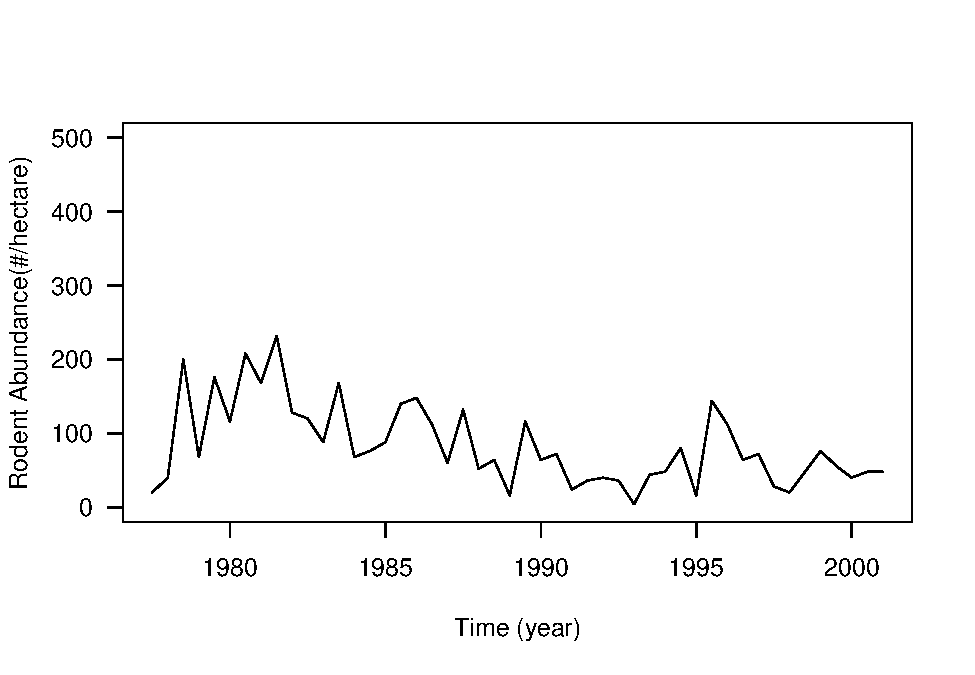
\includegraphics{temporal_assignment_files/figure-latex/unnamed-chunk-4-1.pdf}

\begin{Shaded}
\begin{Highlighting}[]
\CommentTok{#smoothing}
\NormalTok{abund.sm <-}\StringTok{ }\KeywordTok{SMA}\NormalTok{(abund$nn, }\DataTypeTok{n =} \DecValTok{5}\NormalTok{)}

\KeywordTok{plot}\NormalTok{(abund.sm, }\DataTypeTok{type =} \StringTok{"l"}\NormalTok{, }\DataTypeTok{col =} \StringTok{"red"}\NormalTok{, }\DataTypeTok{ylab =} \StringTok{"Rodent Abundance (#/hectare)"}\NormalTok{,}
     \DataTypeTok{xlab =} \StringTok{"Sample"}\NormalTok{, }\DataTypeTok{las =} \DecValTok{1}\NormalTok{, }\DataTypeTok{ylim =} \KeywordTok{c}\NormalTok{(}\DecValTok{0}\NormalTok{, }\DecValTok{500}\NormalTok{))}

\KeywordTok{lines}\NormalTok{(abund$nn, }\DataTypeTok{col =} \StringTok{"black"}\NormalTok{)}

\KeywordTok{legend}\NormalTok{(}\DecValTok{0}\NormalTok{, }\DecValTok{475}\NormalTok{, }\DataTypeTok{col =} \KeywordTok{c}\NormalTok{(}\StringTok{"red"}\NormalTok{, }\StringTok{"black"}\NormalTok{), }\DataTypeTok{lty =} \KeywordTok{c}\NormalTok{(}\DecValTok{1}\NormalTok{,}\DecValTok{1}\NormalTok{),}
       \KeywordTok{c}\NormalTok{(}\StringTok{"smooth"}\NormalTok{, }\StringTok{"non-smooth"}\NormalTok{), }\DataTypeTok{bty =} \StringTok{"n"}\NormalTok{, }\DataTypeTok{cex =} \DecValTok{1}\NormalTok{)}
\end{Highlighting}
\end{Shaded}

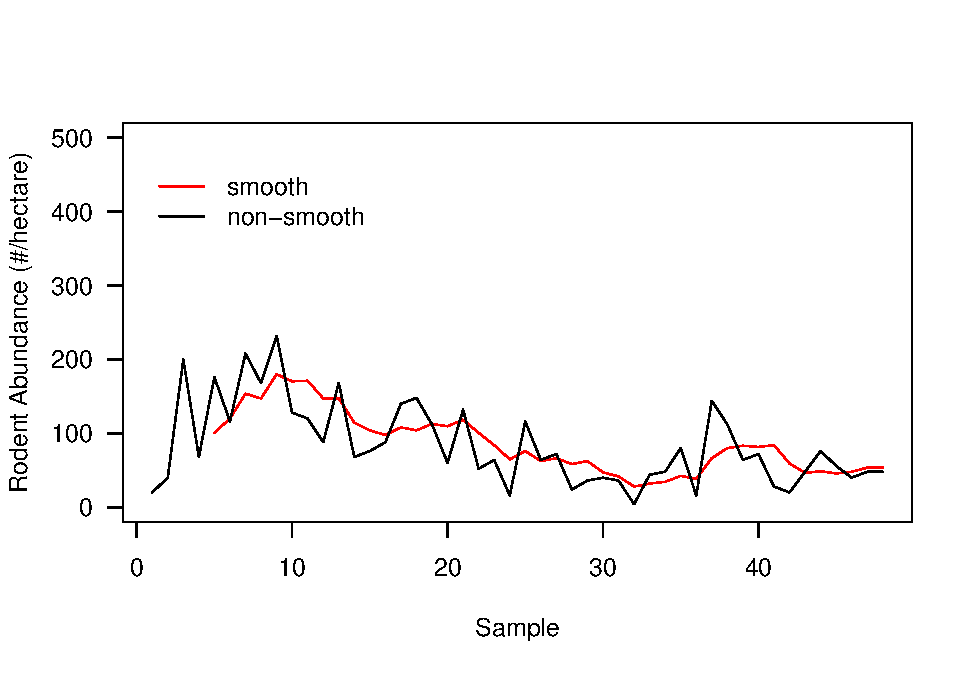
\includegraphics{temporal_assignment_files/figure-latex/unnamed-chunk-4-2.pdf}

\begin{Shaded}
\begin{Highlighting}[]
\CommentTok{#exponential smoothing}
\NormalTok{abund.hw <-}\StringTok{ }\KeywordTok{HoltWinters}\NormalTok{(abund$nn, }\DataTypeTok{beta =} \OtherTok{FALSE}\NormalTok{, }\DataTypeTok{gamma =} \OtherTok{FALSE}\NormalTok{)}

\KeywordTok{plot}\NormalTok{(abund.hw, }\DataTypeTok{xlab =} \StringTok{"Time (year)"}\NormalTok{, }\DataTypeTok{ylim =} \KeywordTok{c}\NormalTok{(}\DecValTok{0}\NormalTok{, }\DecValTok{500}\NormalTok{),}
     \DataTypeTok{ylab =} \StringTok{"Rodent Abundance (#/hectrare)"}\NormalTok{, }\DataTypeTok{las =} \DecValTok{1}\NormalTok{, }\DataTypeTok{main =} \OtherTok{NA}\NormalTok{)}

\KeywordTok{legend}\NormalTok{(}\DecValTok{0}\NormalTok{, }\DecValTok{475}\NormalTok{, }\DataTypeTok{col =} \KeywordTok{c}\NormalTok{(}\StringTok{"black"}\NormalTok{, }\StringTok{"red"}\NormalTok{), }\DataTypeTok{lty =} \KeywordTok{c}\NormalTok{(}\DecValTok{1}\NormalTok{,}\DecValTok{1}\NormalTok{),}
       \KeywordTok{c}\NormalTok{(}\StringTok{"non-smooth"}\NormalTok{, }\StringTok{"smooth"}\NormalTok{), }\DataTypeTok{bty =} \StringTok{"n"}\NormalTok{, }\DataTypeTok{cex =} \DecValTok{1}\NormalTok{)}
\end{Highlighting}
\end{Shaded}

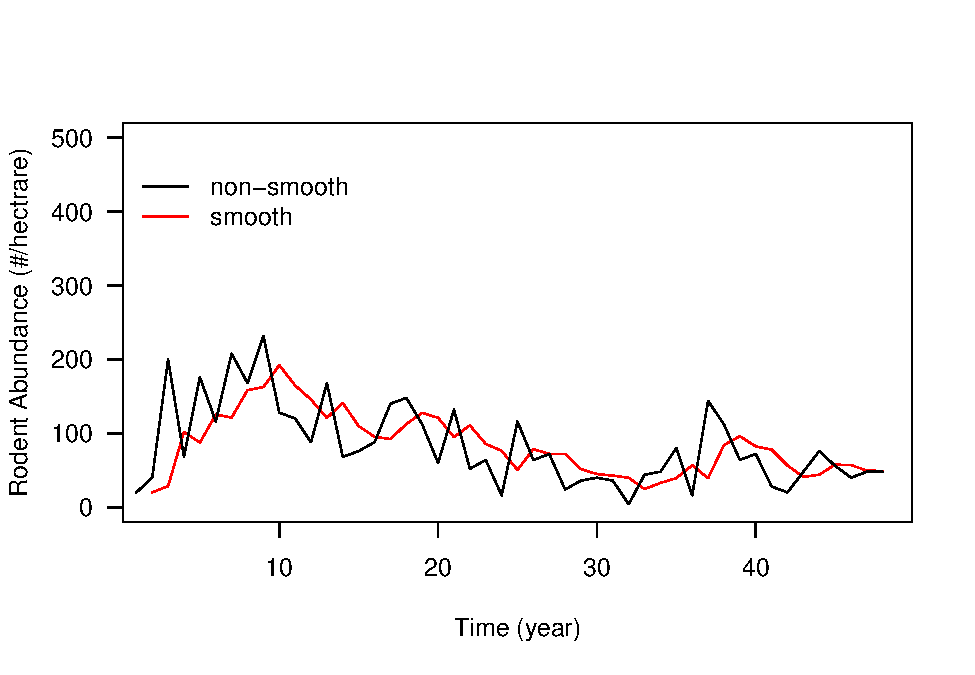
\includegraphics{temporal_assignment_files/figure-latex/unnamed-chunk-4-3.pdf}

\begin{Shaded}
\begin{Highlighting}[]
\CommentTok{#decomposition}
\NormalTok{abund.comp <-}\StringTok{ }\KeywordTok{decompose}\NormalTok{(abund.ts)}
\KeywordTok{plot}\NormalTok{(abund.comp)}
\end{Highlighting}
\end{Shaded}

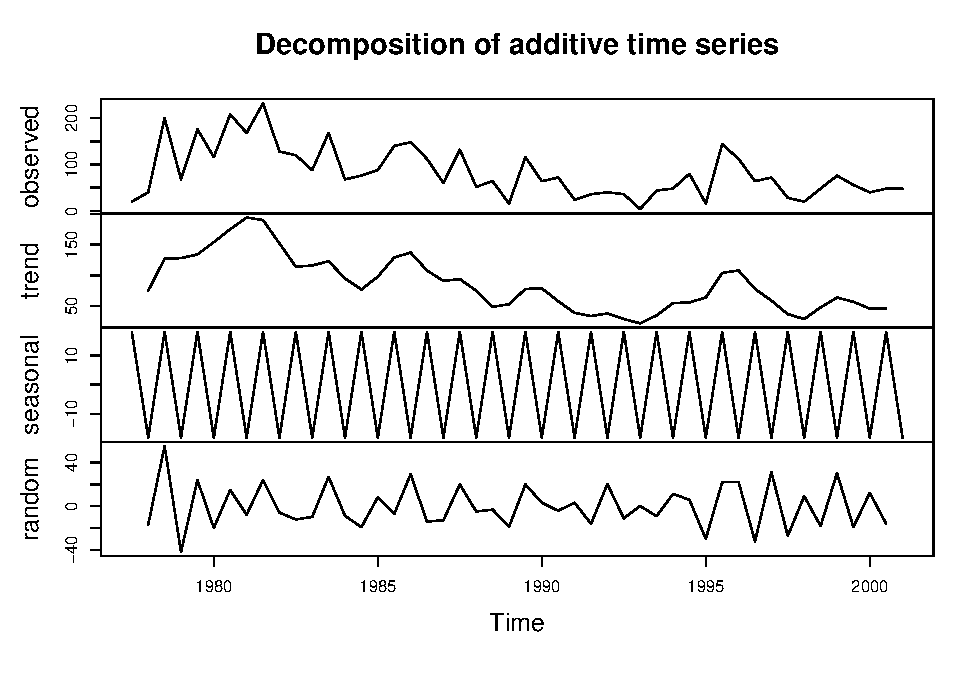
\includegraphics{temporal_assignment_files/figure-latex/unnamed-chunk-4-4.pdf}

\begin{Shaded}
\begin{Highlighting}[]
\NormalTok{abund.adj <-}\StringTok{ }\NormalTok{abund.ts -}\StringTok{ }\NormalTok{abund.comp$seasonal}

\CommentTok{#stationarity}

\NormalTok{adf.raw <-}\StringTok{ }\KeywordTok{adf.test}\NormalTok{(abund.ts, }\DataTypeTok{alternative =} \StringTok{"stationary"}\NormalTok{)}
\NormalTok{adf.raw$p.value}
\end{Highlighting}
\end{Shaded}

\begin{verbatim}
## [1] 0.2547674
\end{verbatim}

\begin{Shaded}
\begin{Highlighting}[]
\NormalTok{abund.ts.diff <-}\StringTok{ }\KeywordTok{diff}\NormalTok{(abund.ts)}
\NormalTok{adf.diff <-}\StringTok{ }\KeywordTok{adf.test}\NormalTok{(abund.ts.diff, }\DataTypeTok{alternative =} \StringTok{"stationary"}\NormalTok{)}
\NormalTok{adf.diff$p.value}
\end{Highlighting}
\end{Shaded}

\begin{verbatim}
## [1] 0.0109537
\end{verbatim}

\begin{Shaded}
\begin{Highlighting}[]
\CommentTok{#pacf and acf}
\KeywordTok{acf}\NormalTok{(abund.ts)}
\end{Highlighting}
\end{Shaded}

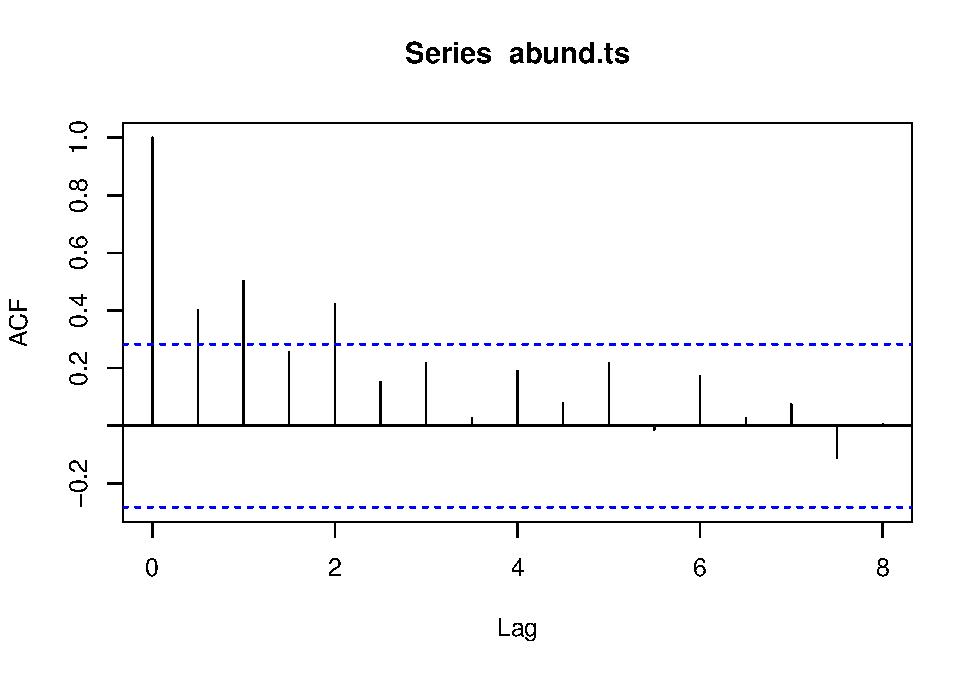
\includegraphics{temporal_assignment_files/figure-latex/unnamed-chunk-4-5.pdf}

\begin{Shaded}
\begin{Highlighting}[]
\KeywordTok{pacf}\NormalTok{(abund.ts)}
\end{Highlighting}
\end{Shaded}

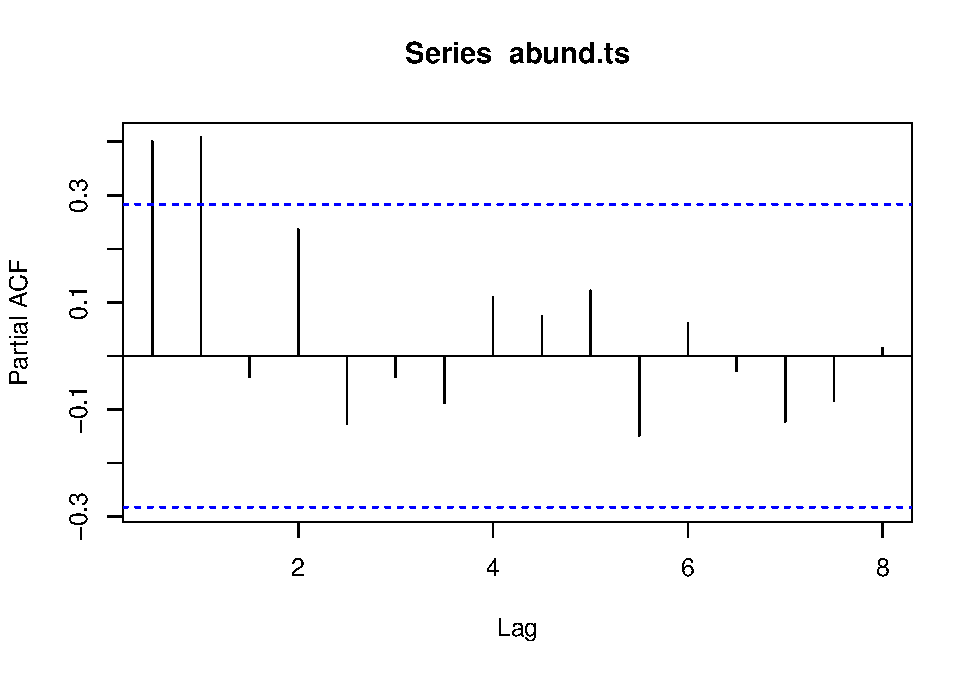
\includegraphics{temporal_assignment_files/figure-latex/unnamed-chunk-4-6.pdf}

\begin{Shaded}
\begin{Highlighting}[]
\CommentTok{#arma}
\NormalTok{abund.arm <-}\StringTok{ }\KeywordTok{auto.arima}\NormalTok{(abund.ts)}
\NormalTok{abund.arm <-}\StringTok{ }\KeywordTok{arima}\NormalTok{((abund.ts), }\KeywordTok{c}\NormalTok{(}\DecValTok{0}\NormalTok{, }\DecValTok{0}\NormalTok{, }\DecValTok{1}\NormalTok{), }\DataTypeTok{seasonal =} \KeywordTok{list}\NormalTok{(}\DataTypeTok{order =} \KeywordTok{c}\NormalTok{(}\DecValTok{2}\NormalTok{, }\DecValTok{1}\NormalTok{, }\DecValTok{0}\NormalTok{),}
                                                           \DataTypeTok{period =} \DecValTok{2}\NormalTok{), }\DataTypeTok{include.mean =}
                     \OtherTok{TRUE}\NormalTok{)}


\KeywordTok{tsdiag}\NormalTok{(abund.arm)}
\end{Highlighting}
\end{Shaded}

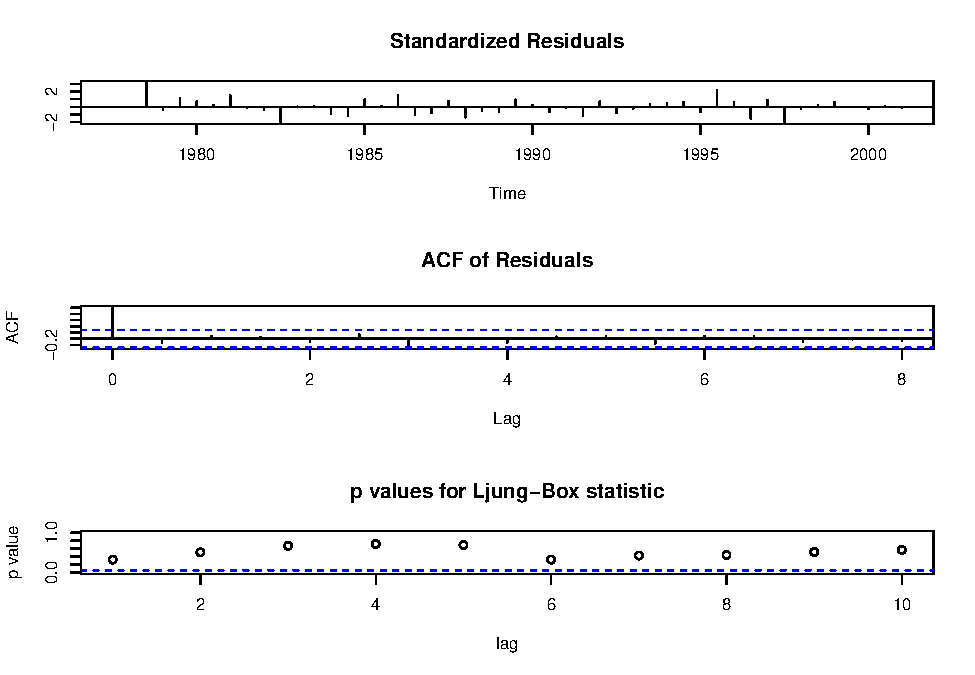
\includegraphics{temporal_assignment_files/figure-latex/unnamed-chunk-4-7.pdf}

\begin{Shaded}
\begin{Highlighting}[]
\NormalTok{pred.arm <-}\StringTok{ }\KeywordTok{predict}\NormalTok{(abund.arm, }\DataTypeTok{n.ahead =} \DecValTok{20}\NormalTok{)}
\KeywordTok{ts.plot}\NormalTok{(abund.ts, pred.arm$pred, }\DataTypeTok{lty =} \KeywordTok{c}\NormalTok{(}\DecValTok{1}\NormalTok{,}\DecValTok{3}\NormalTok{))}
\end{Highlighting}
\end{Shaded}

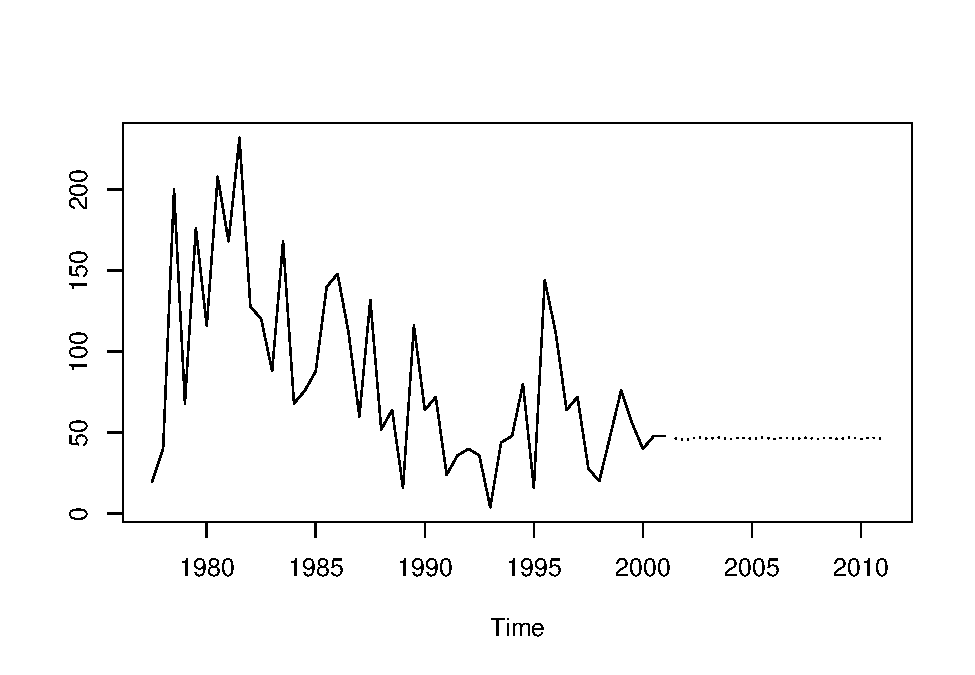
\includegraphics{temporal_assignment_files/figure-latex/unnamed-chunk-4-8.pdf}

\textbf{\emph{Question 3}}: Describe the results from your time series
analysis.

\begin{enumerate}
\def\labelenumi{\alph{enumi}.}
\tightlist
\item
  Does your data meet the assumption of stationarity? If not, what does
  this violation imply?
\item
  What does the ACF function do and how does it relate to the ARMA
  model? How does this differ from PACF?
\item
  What results can you conclude from your full ARMA model along with
  other methods outlined in the time series setcion of the Handout?
\end{enumerate}

\begin{quote}
\textbf{\emph{Answer 3a}}: The data did not meet the assumption of
similarity based on the Dicky-Fuller test (p = 0.25). Hoever, after
differencing the time series, it did meet the assumption of stationarity
(p \textless{} 0.05). \textbf{\emph{Answer 3b}}: ACF is the
autocorreltion function and it lets the researcher determines correltion
that may be inconspicuously located time series intervals. This relates
to the ARMA models because it can help paramatize the model so it can
generate more informative forcasts. Unlike AFC which looks for lagtime
correlations arcoss the data, PACF looks for correlation lagtimes
between two time intervals. Essentially, the AFC measures
autocorrelation in the `MA' (moving average) portion of the ARMA models
and PACF measure autocorrelation in the `AF' (autoreggresive) portion of
the model. \textbf{\emph{Answer 3c}}: Based on the model conclusions,
rodent abundance increased after the plot was established then steadily
decresaed and will likely stablize at a relatively low density through
the future.
\end{quote}

\subsection{5) REPEATED MEASURES ANALYSIS OF VARIANCE
(RM-ANOVA)}\label{repeated-measures-analysis-of-variance-rm-anova}

In the R code chunk below, do the following:

\begin{enumerate}
\def\labelenumi{\arabic{enumi}.}
\tightlist
\item
  Create an appropriate data frame for RM-ANOVA (e.g., yearly species
  abundance values within plots).
\item
  Calculate the inverse of Simpson's diversity for each year, and plot
  it as a function of year for the Control and Rodent Exclosure plots.
\item
  Perform an RM-ANOVA and construct a F-test using the AR(1), compound
  symmetery, and unstructured covariance structures.
\end{enumerate}

\begin{Shaded}
\begin{Highlighting}[]
\NormalTok{##Wrangling data}
\CommentTok{# time-by-species matrix}
\NormalTok{time.by.species <-}\StringTok{ }\KeywordTok{group_by}\NormalTok{(portal, year, plot_id,}
                            \NormalTok{plot_type) %>%}\StringTok{ }\KeywordTok{count}\NormalTok{(taxon) %>%}\StringTok{ }\KeywordTok{spread}\NormalTok{(}\DataTypeTok{key =} \NormalTok{taxon, }\DataTypeTok{value =} \NormalTok{n,}
                                                                   \DataTypeTok{fill =} \DecValTok{0}\NormalTok{)}

\CommentTok{# observed richness from time-by-species matrix}
\NormalTok{richness <-}\StringTok{ }\KeywordTok{as.data.frame}\NormalTok{(}\KeywordTok{rowSums}\NormalTok{(time.by.species[,-}\KeywordTok{c}\NormalTok{(}\DecValTok{1}\NormalTok{:}\DecValTok{3}\NormalTok{)] >}\StringTok{ }\DecValTok{0}\NormalTok{))}

\CommentTok{# data frame with experimental design and richness data}
\NormalTok{rich.all <-}\StringTok{ }\KeywordTok{data.frame}\NormalTok{(time.by.species[,}\DecValTok{1}\NormalTok{:}\DecValTok{3}\NormalTok{,], richness)}

\CommentTok{# Rename column}
\KeywordTok{names}\NormalTok{(rich.all)[}\DecValTok{4}\NormalTok{] <-}\StringTok{ "richness"}


\CommentTok{# Pull out two of the five Portal treatments}
\NormalTok{rich.treat <-}\StringTok{ }\NormalTok{rich.all[}\KeywordTok{which}\NormalTok{(rich.all$plot_type ==}
\StringTok{                               "Control"} \NormalTok{|}\StringTok{ }\NormalTok{rich.all$plot_type ==}\StringTok{ "Rodent Exclosure"}\NormalTok{), ]}

\NormalTok{##Plotting data}
\NormalTok{rich.treat.plot <-}\StringTok{ }\KeywordTok{group_by}\NormalTok{(rich.treat, plot_type, year) %>%}
\StringTok{  }\KeywordTok{summarise}\NormalTok{(}
    \DataTypeTok{mean =} \KeywordTok{mean}\NormalTok{(richness), }
    \DataTypeTok{sd =} \KeywordTok{sd}\NormalTok{(richness), }
    \DataTypeTok{n =} \KeywordTok{n}\NormalTok{(), }
    \DataTypeTok{sem =} \NormalTok{sd/}\KeywordTok{sqrt}\NormalTok{(n)) }

\NormalTok{rich.plot <-}\StringTok{ }\KeywordTok{ggplot}\NormalTok{(rich.treat.plot, }\KeywordTok{aes}\NormalTok{(}\DataTypeTok{x =} \NormalTok{year, }\DataTypeTok{y =} \NormalTok{mean, }\DataTypeTok{color =} \NormalTok{plot_type)) +}
\StringTok{  }\KeywordTok{geom_line}\NormalTok{(}\DataTypeTok{size =} \DecValTok{1}\NormalTok{, }\DataTypeTok{show.legend =} \NormalTok{T) +}
\StringTok{  }\KeywordTok{geom_errorbar}\NormalTok{(}\KeywordTok{aes}\NormalTok{(}\DataTypeTok{ymin =} \NormalTok{mean -}\StringTok{ }\NormalTok{sem, }\DataTypeTok{ymax =} \NormalTok{mean +}\StringTok{ }\NormalTok{sem), }\DataTypeTok{width =} \NormalTok{.}\DecValTok{1}\NormalTok{) +}
\StringTok{  }\KeywordTok{xlim}\NormalTok{(}\DecValTok{1977}\NormalTok{, }\DecValTok{2002}\NormalTok{) +}
\StringTok{  }\KeywordTok{xlab}\NormalTok{(}\StringTok{"Year"}\NormalTok{) +}
\StringTok{  }\KeywordTok{ylab}\NormalTok{(}\StringTok{"Richness"}\NormalTok{)+}
\StringTok{  }\KeywordTok{scale_color_grey}\NormalTok{()}

\KeywordTok{plot}\NormalTok{(rich.plot)}
\end{Highlighting}
\end{Shaded}

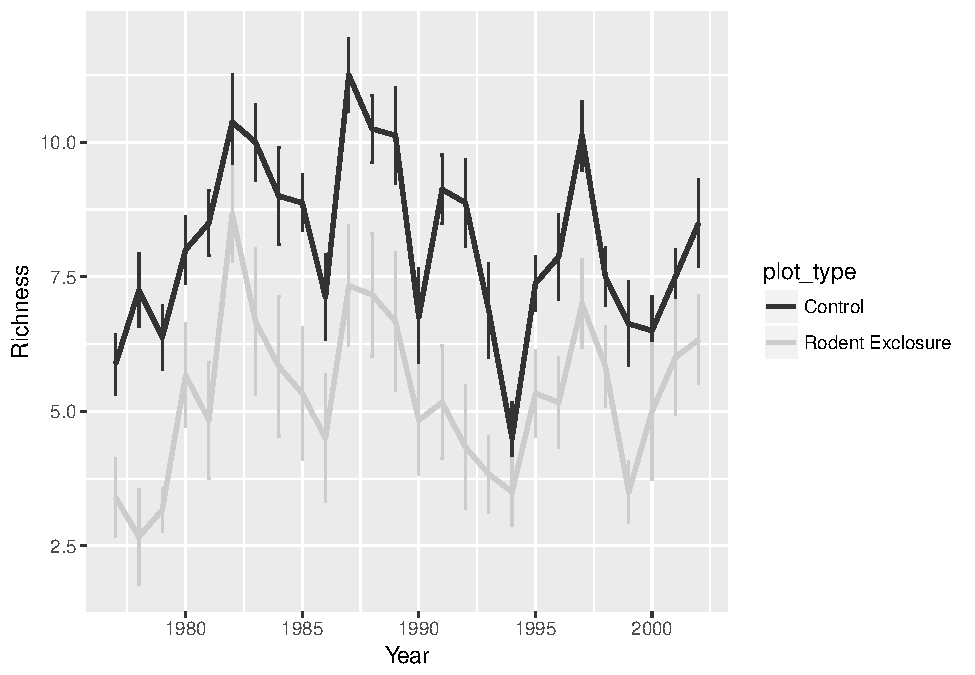
\includegraphics{temporal_assignment_files/figure-latex/unnamed-chunk-5-1.pdf}

\begin{Shaded}
\begin{Highlighting}[]
\CommentTok{#autoregressive}
\NormalTok{rich.rm <-}\StringTok{ }\KeywordTok{lme}\NormalTok{(richness ~}\StringTok{ }\NormalTok{plot_type *}\StringTok{ }\NormalTok{year, }\DataTypeTok{random =} \NormalTok{~}\StringTok{ }\DecValTok{1} \NormalTok{|}\StringTok{ }\NormalTok{plot_id,}
               \DataTypeTok{correlation =} \KeywordTok{corAR1}\NormalTok{(}\DataTypeTok{form =} \NormalTok{~}\StringTok{ }\DecValTok{1} \NormalTok{|}\StringTok{ }\NormalTok{plot_id),}
               \DataTypeTok{data =} \NormalTok{rich.treat)}
\KeywordTok{summary}\NormalTok{(rich.rm)}
\end{Highlighting}
\end{Shaded}

\begin{verbatim}
## Linear mixed-effects model fit by REML
##  Data: rich.treat 
##        AIC      BIC    logLik
##   1590.462 1617.567 -788.2309
## 
## Random effects:
##  Formula: ~1 | plot_id
##         (Intercept) Residual
## StdDev:    1.296979 2.246238
## 
## Correlation Structure: AR(1)
##  Formula: ~1 | plot_id 
##  Parameter estimate(s):
##     Phi 
## 0.37097 
## Fixed effects: richness ~ plot_type * year 
##                                    Value Std.Error  DF    t-value p-value
## (Intercept)                     28.62737  57.07705 343  0.5015565  0.6163
## plot_typeRodent Exclosure      -62.03957  89.14103  12 -0.6959710  0.4997
## year                            -0.01033   0.02869 343 -0.3600129  0.7191
## plot_typeRodent Exclosure:year   0.02980   0.04480 343  0.6652702  0.5063
##  Correlation: 
##                                (Intr) plt_RE year 
## plot_typeRodent Exclosure      -0.64              
## year                           -1.00   0.64       
## plot_typeRodent Exclosure:year  0.64  -1.00  -0.64
## 
## Standardized Within-Group Residuals:
##         Min          Q1         Med          Q3         Max 
## -2.98978687 -0.69549540 -0.07250359  0.68791058  2.73090608 
## 
## Number of Observations: 359
## Number of Groups: 14
\end{verbatim}

\begin{Shaded}
\begin{Highlighting}[]
\KeywordTok{anova}\NormalTok{(rich.rm)}
\end{Highlighting}
\end{Shaded}

\begin{verbatim}
##                numDF denDF  F-value p-value
## (Intercept)        1   343 319.5050  <.0001
## plot_type          1    12  12.2775  0.0044
## year               1   343   0.0074  0.9316
## plot_type:year     1   343   0.4426  0.5063
\end{verbatim}

\begin{Shaded}
\begin{Highlighting}[]
\KeywordTok{set.caption}\NormalTok{(}\StringTok{"RMANOVA for Portal"}\NormalTok{)}
\KeywordTok{pander}\NormalTok{(}\KeywordTok{anova}\NormalTok{(rich.rm))}
\end{Highlighting}
\end{Shaded}

\begin{longtable}[]{@{}ccccc@{}}
\caption{RMANOVA for Portal}\tabularnewline
\toprule
\begin{minipage}[b]{0.25\columnwidth}\centering\strut
~\strut
\end{minipage} & \begin{minipage}[b]{0.10\columnwidth}\centering\strut
numDF\strut
\end{minipage} & \begin{minipage}[b]{0.10\columnwidth}\centering\strut
denDF\strut
\end{minipage} & \begin{minipage}[b]{0.12\columnwidth}\centering\strut
F-value\strut
\end{minipage} & \begin{minipage}[b]{0.12\columnwidth}\centering\strut
p-value\strut
\end{minipage}\tabularnewline
\midrule
\endfirsthead
\toprule
\begin{minipage}[b]{0.25\columnwidth}\centering\strut
~\strut
\end{minipage} & \begin{minipage}[b]{0.10\columnwidth}\centering\strut
numDF\strut
\end{minipage} & \begin{minipage}[b]{0.10\columnwidth}\centering\strut
denDF\strut
\end{minipage} & \begin{minipage}[b]{0.12\columnwidth}\centering\strut
F-value\strut
\end{minipage} & \begin{minipage}[b]{0.12\columnwidth}\centering\strut
p-value\strut
\end{minipage}\tabularnewline
\midrule
\endhead
\begin{minipage}[t]{0.25\columnwidth}\centering\strut
\textbf{(Intercept)}\strut
\end{minipage} & \begin{minipage}[t]{0.10\columnwidth}\centering\strut
1\strut
\end{minipage} & \begin{minipage}[t]{0.10\columnwidth}\centering\strut
343\strut
\end{minipage} & \begin{minipage}[t]{0.12\columnwidth}\centering\strut
319.5\strut
\end{minipage} & \begin{minipage}[t]{0.12\columnwidth}\centering\strut
0\strut
\end{minipage}\tabularnewline
\begin{minipage}[t]{0.25\columnwidth}\centering\strut
\textbf{plot\_type}\strut
\end{minipage} & \begin{minipage}[t]{0.10\columnwidth}\centering\strut
1\strut
\end{minipage} & \begin{minipage}[t]{0.10\columnwidth}\centering\strut
12\strut
\end{minipage} & \begin{minipage}[t]{0.12\columnwidth}\centering\strut
12.28\strut
\end{minipage} & \begin{minipage}[t]{0.12\columnwidth}\centering\strut
0.00435\strut
\end{minipage}\tabularnewline
\begin{minipage}[t]{0.25\columnwidth}\centering\strut
\textbf{year}\strut
\end{minipage} & \begin{minipage}[t]{0.10\columnwidth}\centering\strut
1\strut
\end{minipage} & \begin{minipage}[t]{0.10\columnwidth}\centering\strut
343\strut
\end{minipage} & \begin{minipage}[t]{0.12\columnwidth}\centering\strut
0.007381\strut
\end{minipage} & \begin{minipage}[t]{0.12\columnwidth}\centering\strut
0.9316\strut
\end{minipage}\tabularnewline
\begin{minipage}[t]{0.25\columnwidth}\centering\strut
\textbf{plot\_type:year}\strut
\end{minipage} & \begin{minipage}[t]{0.10\columnwidth}\centering\strut
1\strut
\end{minipage} & \begin{minipage}[t]{0.10\columnwidth}\centering\strut
343\strut
\end{minipage} & \begin{minipage}[t]{0.12\columnwidth}\centering\strut
0.4426\strut
\end{minipage} & \begin{minipage}[t]{0.12\columnwidth}\centering\strut
0.5063\strut
\end{minipage}\tabularnewline
\bottomrule
\end{longtable}

\begin{Shaded}
\begin{Highlighting}[]
\KeywordTok{lsmeans}\NormalTok{(rich.rm, ~plot_type)}
\end{Highlighting}
\end{Shaded}

\begin{verbatim}
## NOTE: Results may be misleading due to involvement in interactions
\end{verbatim}

\begin{verbatim}
##  plot_type          lsmean        SE df lower.CL upper.CL
##  Control          8.078695 0.5107372 13 6.975315 9.182076
##  Rodent Exclosure 5.338471 0.5916197 12 4.049442 6.627499
## 
## Confidence level used: 0.95
\end{verbatim}

\begin{Shaded}
\begin{Highlighting}[]
\CommentTok{#unstructured}
\CommentTok{#rich.rmuns <- lme(richness ~ plot_type * year, random = ~ plot_type * year | plot_id, data = rich.treat,correlation = corSymm(form = ~ 1 | plot_id), control = lmeControl(opt='optim'))}


\CommentTok{#compound symmetry}
\NormalTok{rich.rmcom <-}\StringTok{ }\KeywordTok{lme}\NormalTok{(richness ~}\StringTok{ }\NormalTok{plot_type *}\StringTok{ }\NormalTok{year, }\DataTypeTok{random =} \NormalTok{~}\StringTok{ }\DecValTok{1} \NormalTok{|}\StringTok{ }\NormalTok{plot_id,}
               \DataTypeTok{correlation =} \KeywordTok{corCompSymm}\NormalTok{(}\DataTypeTok{form =} \NormalTok{~}\StringTok{ }\DecValTok{1} \NormalTok{|}\StringTok{ }\NormalTok{plot_id),}
               \DataTypeTok{data =} \NormalTok{rich.treat)}
\KeywordTok{summary}\NormalTok{(rich.rmcom)}
\end{Highlighting}
\end{Shaded}

\begin{verbatim}
## Linear mixed-effects model fit by REML
##  Data: rich.treat 
##        AIC      BIC    logLik
##   1634.628 1661.733 -810.3142
## 
## Random effects:
##  Formula: ~1 | plot_id
##         (Intercept) Residual
## StdDev:    1.395556 2.185797
## 
## Correlation Structure: Compound symmetry
##  Formula: ~1 | plot_id 
##  Parameter estimate(s):
##          Rho 
## 6.672013e-18 
## Fixed effects: richness ~ plot_type * year 
##                                    Value Std.Error  DF   t-value p-value
## (Intercept)                     61.25855  40.20654 343  1.523597  0.1285
## plot_typeRodent Exclosure      -66.04270  62.95273  12 -1.049084  0.3148
## year                            -0.02671   0.02021 343 -1.321744  0.1871
## plot_typeRodent Exclosure:year   0.03181   0.03164 343  1.005341  0.3154
##  Correlation: 
##                                (Intr) plt_RE year  
## plot_typeRodent Exclosure      -0.639              
## year                           -1.000  0.639       
## plot_typeRodent Exclosure:year  0.639 -1.000 -0.639
## 
## Standardized Within-Group Residuals:
##        Min         Q1        Med         Q3        Max 
## -3.0806434 -0.6993469 -0.0728110  0.6795500  2.7655354 
## 
## Number of Observations: 359
## Number of Groups: 14
\end{verbatim}

\begin{Shaded}
\begin{Highlighting}[]
\KeywordTok{anova}\NormalTok{(rich.rmcom)}
\end{Highlighting}
\end{Shaded}

\begin{verbatim}
##                numDF denDF   F-value p-value
## (Intercept)        1   343 315.82853  <.0001
## plot_type          1    12  12.25170  0.0044
## year               1   343   0.78014  0.3777
## plot_type:year     1   343   1.01071  0.3154
\end{verbatim}

\begin{Shaded}
\begin{Highlighting}[]
\KeywordTok{set.caption}\NormalTok{(}\StringTok{"RMANOVA for Portal"}\NormalTok{)}
\KeywordTok{pander}\NormalTok{(}\KeywordTok{anova}\NormalTok{(rich.rmcom))}
\end{Highlighting}
\end{Shaded}

\begin{longtable}[]{@{}ccccc@{}}
\caption{RMANOVA for Portal}\tabularnewline
\toprule
\begin{minipage}[b]{0.25\columnwidth}\centering\strut
~\strut
\end{minipage} & \begin{minipage}[b]{0.10\columnwidth}\centering\strut
numDF\strut
\end{minipage} & \begin{minipage}[b]{0.10\columnwidth}\centering\strut
denDF\strut
\end{minipage} & \begin{minipage}[b]{0.12\columnwidth}\centering\strut
F-value\strut
\end{minipage} & \begin{minipage}[b]{0.12\columnwidth}\centering\strut
p-value\strut
\end{minipage}\tabularnewline
\midrule
\endfirsthead
\toprule
\begin{minipage}[b]{0.25\columnwidth}\centering\strut
~\strut
\end{minipage} & \begin{minipage}[b]{0.10\columnwidth}\centering\strut
numDF\strut
\end{minipage} & \begin{minipage}[b]{0.10\columnwidth}\centering\strut
denDF\strut
\end{minipage} & \begin{minipage}[b]{0.12\columnwidth}\centering\strut
F-value\strut
\end{minipage} & \begin{minipage}[b]{0.12\columnwidth}\centering\strut
p-value\strut
\end{minipage}\tabularnewline
\midrule
\endhead
\begin{minipage}[t]{0.25\columnwidth}\centering\strut
\textbf{(Intercept)}\strut
\end{minipage} & \begin{minipage}[t]{0.10\columnwidth}\centering\strut
1\strut
\end{minipage} & \begin{minipage}[t]{0.10\columnwidth}\centering\strut
343\strut
\end{minipage} & \begin{minipage}[t]{0.12\columnwidth}\centering\strut
315.8\strut
\end{minipage} & \begin{minipage}[t]{0.12\columnwidth}\centering\strut
0\strut
\end{minipage}\tabularnewline
\begin{minipage}[t]{0.25\columnwidth}\centering\strut
\textbf{plot\_type}\strut
\end{minipage} & \begin{minipage}[t]{0.10\columnwidth}\centering\strut
1\strut
\end{minipage} & \begin{minipage}[t]{0.10\columnwidth}\centering\strut
12\strut
\end{minipage} & \begin{minipage}[t]{0.12\columnwidth}\centering\strut
12.25\strut
\end{minipage} & \begin{minipage}[t]{0.12\columnwidth}\centering\strut
0.00438\strut
\end{minipage}\tabularnewline
\begin{minipage}[t]{0.25\columnwidth}\centering\strut
\textbf{year}\strut
\end{minipage} & \begin{minipage}[t]{0.10\columnwidth}\centering\strut
1\strut
\end{minipage} & \begin{minipage}[t]{0.10\columnwidth}\centering\strut
343\strut
\end{minipage} & \begin{minipage}[t]{0.12\columnwidth}\centering\strut
0.7801\strut
\end{minipage} & \begin{minipage}[t]{0.12\columnwidth}\centering\strut
0.3777\strut
\end{minipage}\tabularnewline
\begin{minipage}[t]{0.25\columnwidth}\centering\strut
\textbf{plot\_type:year}\strut
\end{minipage} & \begin{minipage}[t]{0.10\columnwidth}\centering\strut
1\strut
\end{minipage} & \begin{minipage}[t]{0.10\columnwidth}\centering\strut
343\strut
\end{minipage} & \begin{minipage}[t]{0.12\columnwidth}\centering\strut
1.011\strut
\end{minipage} & \begin{minipage}[t]{0.12\columnwidth}\centering\strut
0.3154\strut
\end{minipage}\tabularnewline
\bottomrule
\end{longtable}

\begin{Shaded}
\begin{Highlighting}[]
\KeywordTok{lsmeans}\NormalTok{(rich.rmcom, ~plot_type)}
\end{Highlighting}
\end{Shaded}

\begin{verbatim}
## NOTE: Results may be misleading due to involvement in interactions
\end{verbatim}

\begin{verbatim}
##  plot_type          lsmean        SE df lower.CL upper.CL
##  Control          8.117551 0.5161597 13 7.002456 9.232646
##  Rodent Exclosure 5.357391 0.5968970 12 4.056865 6.657918
## 
## Confidence level used: 0.95
\end{verbatim}

\textbf{\emph{Question 4}}: Describe the results from your RM-ANOVA.

\begin{enumerate}
\def\labelenumi{\alph{enumi}.}
\tightlist
\item
  In your own words describe what a RM-ANOVA test is doing
\item
  Is there a noticeable trend in the inverse of Simpson's diversity over
  time?
\item
  What does the result of your F-test tell you?
\item
  Of the three RM-ANOVA models with different covariance structures,
  which one is best? How does this affect the interpretation of your
  data?
\end{enumerate}

\begin{quote}
\textbf{\emph{Answer 4a}}: It is testing the effect of plot\_type, year,
and the interaction between plot\_type and year on the response variable
(rodent richness). It is basically a regular ANOVA, but for
nonindependent groups. In this example, we are testing for differences
in intercept (time) since we don't have an a priori reason to test
intercept-slope model.\\
\textbf{\emph{Answer 4b}}: Based on eyeballing the plot, it seems as if
there might be a slight increase of richness over time and the two plot
types seems to follow the same general trends (however this may be due
to environmental changes). \textbf{\emph{Answer 4c}}: Plot\_type has a
significant effect on rodent richness (F = 12.28, df = 1/12, p
\textless{} 0.01). Neither year (F = 0.01, df = 1/343, p = 0.93) nor the
interaction between year and plot\_type (F = 0.45, df = 1/343, p = 0.51)
have a significant effect on rodent richness. Therefore, there is a
significant difference in richness over time when you compare full
rodent exclosure from a plot and full rodent access to a plot, and this
is most fully explained by the plot\_type treatment. In general, based
on the F values treatment means only considerably differ between plot
types. \textbf{\emph{Answer 4d}}: The autoregressive model appeared to
work the best. This would say that the time intercept is a good measure
of diversity change over time.
\end{quote}

\subsection{6) TEMPORAL BETA DIVERSITY}\label{temporal-beta-diversity}

\subsubsection{Turnover}\label{turnover}

In the R code chunk below, do the following:

\begin{enumerate}
\def\labelenumi{\arabic{enumi}.}
\tightlist
\item
  Calculate species abundances for each taxonomic group (the
  \texttt{taxa} column).
\item
  Calculate total turnover and turnover due to the gain/loss of species
  for each group.
\item
  Visualize turnover within each group
\end{enumerate}

\begin{Shaded}
\begin{Highlighting}[]
\NormalTok{portal.species.abunds <-}\StringTok{ }\KeywordTok{group_by}\NormalTok{(portal, year, plot_type) %>%}\StringTok{ }\KeywordTok{count}\NormalTok{(taxon)}

\NormalTok{portal.total <-}\StringTok{ }\KeywordTok{turnover}\NormalTok{(}\DataTypeTok{df =} \NormalTok{portal.species.abunds,}
                         \DataTypeTok{time.var =} \StringTok{"year"}\NormalTok{,}
                         \DataTypeTok{species.var =} \StringTok{"taxon"}\NormalTok{,}
                         \DataTypeTok{abundance.var =} \StringTok{"n"}\NormalTok{,}
                         \DataTypeTok{replicate.var =} \StringTok{"plot_type"}\NormalTok{,}
                         \DataTypeTok{metric =} \StringTok{"total"}\NormalTok{)}

\NormalTok{portal.appearance <-}\StringTok{ }\KeywordTok{turnover}\NormalTok{(}\DataTypeTok{df =} \NormalTok{portal.species.abunds,}
                              \DataTypeTok{time.var =} \StringTok{"year"}\NormalTok{,}
                              \DataTypeTok{species.var =} \StringTok{"taxon"}\NormalTok{,}
                              \DataTypeTok{abundance.var =} \StringTok{"n"}\NormalTok{,}
                              \DataTypeTok{replicate.var =} \StringTok{"plot_type"}\NormalTok{,}
                              \DataTypeTok{metric =} \StringTok{"appearance"}\NormalTok{)}

\NormalTok{portal.disappearance <-}\StringTok{ }\KeywordTok{turnover}\NormalTok{(}\DataTypeTok{df =} \NormalTok{portal.species.abunds,}
                                 \DataTypeTok{time.var =} \StringTok{"year"}\NormalTok{,}
                                 \DataTypeTok{species.var =} \StringTok{"taxon"}\NormalTok{,}
                                 \DataTypeTok{abundance.var =} \StringTok{"n"}\NormalTok{,}
                                 \DataTypeTok{replicate.var =} \StringTok{"plot_type"}\NormalTok{,}
                                 \DataTypeTok{metric =} \StringTok{"disappearance"}\NormalTok{)}

\NormalTok{portal.turnover <-}\StringTok{ }\KeywordTok{full_join}\NormalTok{(portal.total, portal.disappearance) %>%}
\StringTok{  }\KeywordTok{full_join}\NormalTok{(portal.appearance)}
\end{Highlighting}
\end{Shaded}

\begin{verbatim}
## Joining, by = c("year", "plot_type")
## Joining, by = c("year", "plot_type")
\end{verbatim}

\begin{Shaded}
\begin{Highlighting}[]
\NormalTok{portal.turnover <-}\StringTok{ }\KeywordTok{gather}\NormalTok{(portal.turnover, }\DataTypeTok{key =} \NormalTok{metric, }\DataTypeTok{value =} \NormalTok{turnover,}
                          \NormalTok{total, appearance, disappearance)}

\NormalTok{turn.plot <-}\StringTok{ }\KeywordTok{ggplot}\NormalTok{(}
  \NormalTok{portal.turnover, }\KeywordTok{aes}\NormalTok{(}\DataTypeTok{x =} \NormalTok{year, }\DataTypeTok{y =} \NormalTok{turnover, }\DataTypeTok{color =} \NormalTok{metric)) +}
\StringTok{  }\KeywordTok{geom_line}\NormalTok{(}\DataTypeTok{size =} \DecValTok{1}\NormalTok{, }\DataTypeTok{show.legend =} \NormalTok{T) +}
\StringTok{  }\KeywordTok{facet_wrap}\NormalTok{(~plot_type, }\DataTypeTok{ncol =} \DecValTok{1}\NormalTok{) +}
\StringTok{  }\KeywordTok{xlim}\NormalTok{(}\DecValTok{1977}\NormalTok{, }\DecValTok{2002}\NormalTok{) +}
\StringTok{  }\KeywordTok{xlab}\NormalTok{(}\StringTok{"Year"}\NormalTok{) +}
\StringTok{  }\KeywordTok{ylab}\NormalTok{(}\StringTok{"Turnover"}\NormalTok{) +}
\StringTok{  }\KeywordTok{theme}\NormalTok{(}\DataTypeTok{legend.position =} \StringTok{"bottom"}\NormalTok{) +}
\StringTok{  }\KeywordTok{scale_color_grey}\NormalTok{()}

\KeywordTok{plot}\NormalTok{(turn.plot)}
\end{Highlighting}
\end{Shaded}

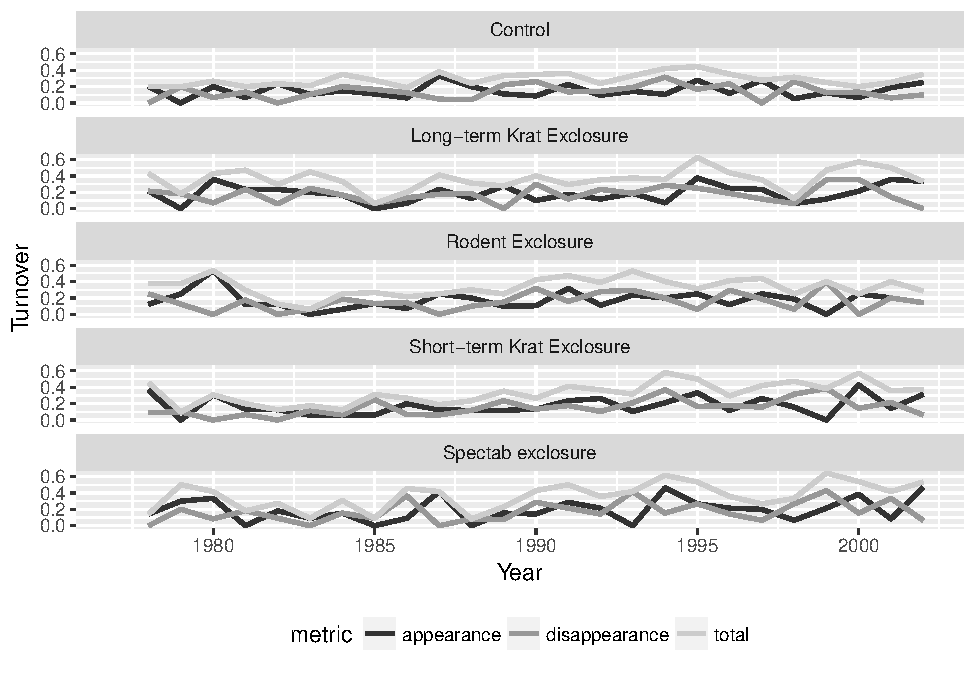
\includegraphics{temporal_assignment_files/figure-latex/unnamed-chunk-6-1.pdf}

\textbf{\emph{Question 5}}:

\begin{enumerate}
\def\labelenumi{\alph{enumi}.}
\tightlist
\item
  How does temporal turnover relate to spatial turnover?\\
\item
  Which taxonomic group appears to be the most variable? Which group
  appears to be the least variable?
\end{enumerate}

\begin{quote}
\textbf{\emph{Answer 5a}}: Time and space are inherently linked in that
changes in space occurr over time. Therefore, it is imporant to consider
temporal and spatial turnover when examining temporal data to better
understand how and why your reponse variable is changing.
\textbf{\emph{Answer 5a}}: The taxonomic group that excludes Dypodomys
spectabilis is the most variable. The control treatment is the least
variable.
\end{quote}

\subsubsection{Mean Rank Shift}\label{mean-rank-shift}

In the code chunk below, do the following:

\begin{enumerate}
\def\labelenumi{\arabic{enumi}.}
\tightlist
\item
  Choose two plot\_types or two plot\_ids and compare the mean rank
  shift (MRS) between them.
\item
  Plot MRS for each through time.
\end{enumerate}

\begin{Shaded}
\begin{Highlighting}[]
\NormalTok{portal.abunds.cont.rodent <-}\StringTok{ }\KeywordTok{filter}\NormalTok{(portal.species.abunds,}
                                    \NormalTok{plot_type ==}\StringTok{ "Control"} \NormalTok{|}\StringTok{ }\NormalTok{plot_type ==}\StringTok{ "Short-term Krat Exclosure"}\NormalTok{)}

\NormalTok{portal.rankshift <-}\StringTok{ }\KeywordTok{rank_shift}\NormalTok{(}
  \DataTypeTok{df =} \KeywordTok{as.data.frame}\NormalTok{(portal.abunds.cont.rodent),}
  \DataTypeTok{time.var =} \StringTok{"year"}\NormalTok{,}
  \DataTypeTok{species.var =} \StringTok{"taxon"}\NormalTok{,}
  \DataTypeTok{abundance.var =} \StringTok{"n"}\NormalTok{,}
  \DataTypeTok{replicate.var =} \StringTok{"plot_type"}\NormalTok{)}

\NormalTok{portal.rankshift$year <-}\StringTok{ }\KeywordTok{as.numeric}\NormalTok{(}\KeywordTok{substr}\NormalTok{(portal.rankshift$year_pair, }\DecValTok{6}\NormalTok{, }\DecValTok{9}\NormalTok{))}

\NormalTok{rankshift.plot <-}\StringTok{ }\KeywordTok{ggplot}\NormalTok{(portal.rankshift, }\KeywordTok{aes}\NormalTok{(}\DataTypeTok{x =} \NormalTok{year, }\DataTypeTok{y =} \NormalTok{MRS, }\DataTypeTok{color =} \NormalTok{plot_type)) +}
\StringTok{  }\KeywordTok{geom_line}\NormalTok{(}\DataTypeTok{size =} \DecValTok{1}\NormalTok{) +}
\StringTok{  }\KeywordTok{xlim}\NormalTok{(}\DecValTok{1977}\NormalTok{, }\DecValTok{2002}\NormalTok{) +}
\StringTok{  }\KeywordTok{xlab}\NormalTok{(}\StringTok{"Year"}\NormalTok{) +}
\StringTok{  }\KeywordTok{ylab}\NormalTok{(}\StringTok{"Mean Rank Shift"}\NormalTok{) +}
\StringTok{  }\KeywordTok{scale_color_grey}\NormalTok{()}

\KeywordTok{plot}\NormalTok{(rankshift.plot)}
\end{Highlighting}
\end{Shaded}

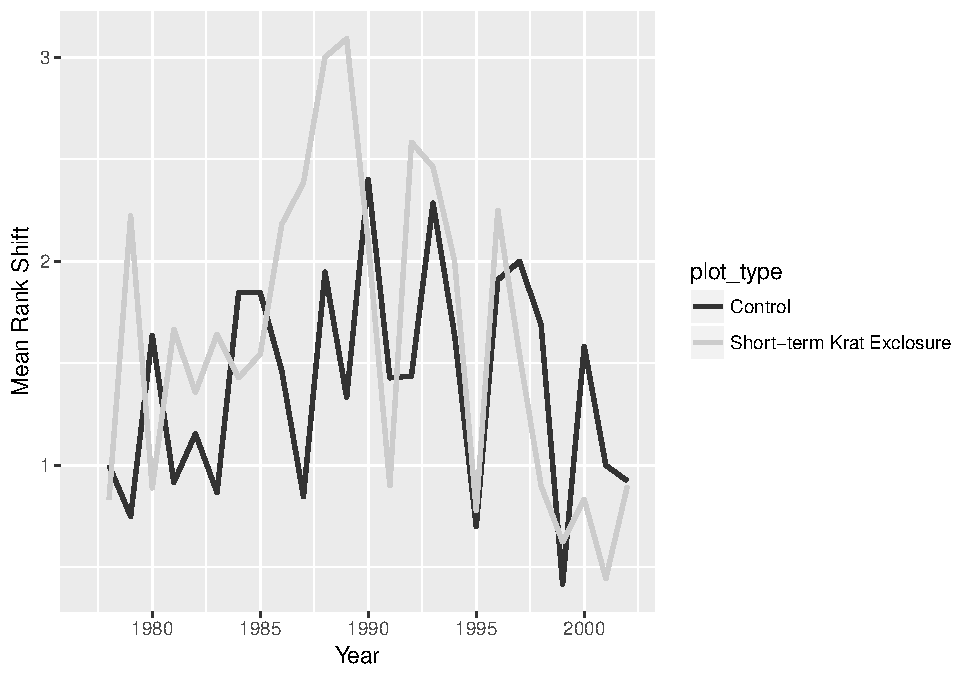
\includegraphics{temporal_assignment_files/figure-latex/unnamed-chunk-7-1.pdf}

\begin{Shaded}
\begin{Highlighting}[]
\KeywordTok{group_by}\NormalTok{(portal.rankshift, plot_type) %>%}
\StringTok{  }\KeywordTok{summarise}\NormalTok{(}
    \DataTypeTok{mean =} \KeywordTok{mean}\NormalTok{(MRS),}
    \DataTypeTok{cv =} \KeywordTok{sd}\NormalTok{(MRS)/mean)}
\end{Highlighting}
\end{Shaded}

\begin{verbatim}
## # A tibble: 2 × 3
##                   plot_type     mean        cv
##                       <chr>    <dbl>     <dbl>
## 1                   Control 1.400675 0.3759483
## 2 Short-term Krat Exclosure 1.622171 0.4751513
\end{verbatim}

\textbf{\emph{Question 6}}:

\begin{enumerate}
\def\labelenumi{\alph{enumi}.}
\tightlist
\item
  What does a change in the rank shift tell you about the community?
\item
  Interpret the analysis and figure you just made.
\end{enumerate}

\begin{quote}
\textbf{\emph{Answer 6a}}: Changes in rank shift provide clues into the
potential influence of groups based on rank abundance; therefore it
accounts for the influence of rare/abundant species based on their rank.
\textbf{\emph{Answer 6b}}: It appears as if the presence of Dipodomys
spp. had an influence on the on abundance. On average MRS is higher in
the Short-Term Krat enclosure (mean = 1.79) than the control enclosure
(mean = 1.40).
\end{quote}

\subsubsection{Rate Change Interval}\label{rate-change-interval}

In the R code chunk below, do the following:

\begin{enumerate}
\def\labelenumi{\arabic{enumi}.}
\tightlist
\item
  Calculate the rate change interval using the Hellinger distance.
\item
  Plot the results.
\end{enumerate}

\begin{Shaded}
\begin{Highlighting}[]
\NormalTok{portal.species.abunds$tot.abund <-}\StringTok{ }\KeywordTok{rep}\NormalTok{(}\KeywordTok{sum}\NormalTok{(portal.species.abunds$n),}
                                       \KeywordTok{length}\NormalTok{(portal.species.abunds$n))}

\NormalTok{portal.hellinger.transf <-}\StringTok{ }\NormalTok{portal.species.abunds %>%}
\StringTok{  }\KeywordTok{mutate}\NormalTok{(}\DataTypeTok{hellinger.transf =} \KeywordTok{sqrt}\NormalTok{(n /}\StringTok{ }\NormalTok{tot.abund))}

\NormalTok{portal.change.int <-}\StringTok{ }\KeywordTok{rate_change_interval}\NormalTok{(portal.hellinger.transf,}
                                          \DataTypeTok{time.var =} \StringTok{"year"}\NormalTok{,}
                                          \DataTypeTok{species.var =} \StringTok{"taxon"}\NormalTok{,}
                                          \DataTypeTok{abundance.var =} \StringTok{"hellinger.transf"}\NormalTok{,}
                                          \DataTypeTok{replicate.var =} \StringTok{"plot_type"}\NormalTok{)}

\NormalTok{rate.plot <-}\StringTok{ }\KeywordTok{ggplot}\NormalTok{(portal.change.int, }\KeywordTok{aes}\NormalTok{(interval, distance)) +}
\StringTok{  }\KeywordTok{geom_point}\NormalTok{() +}
\StringTok{  }\KeywordTok{facet_wrap}\NormalTok{(~plot_type) +}
\StringTok{  }\KeywordTok{theme}\NormalTok{(}\DataTypeTok{strip.text.x =} \KeywordTok{element_text}\NormalTok{(}\DataTypeTok{size =} \DecValTok{7}\NormalTok{)) +}
\StringTok{  }\KeywordTok{stat_smooth}\NormalTok{(}\DataTypeTok{method =} \StringTok{"loess"}\NormalTok{, }\DataTypeTok{se =} \NormalTok{F, }\DataTypeTok{size =} \DecValTok{1}\NormalTok{) +}
\StringTok{  }\KeywordTok{ylab}\NormalTok{(}\StringTok{"Hellinger Distance"}\NormalTok{) +}
\StringTok{  }\KeywordTok{xlab}\NormalTok{(}\StringTok{"Time Interval (Years)"}\NormalTok{)}

\NormalTok{rate.plot}
\end{Highlighting}
\end{Shaded}

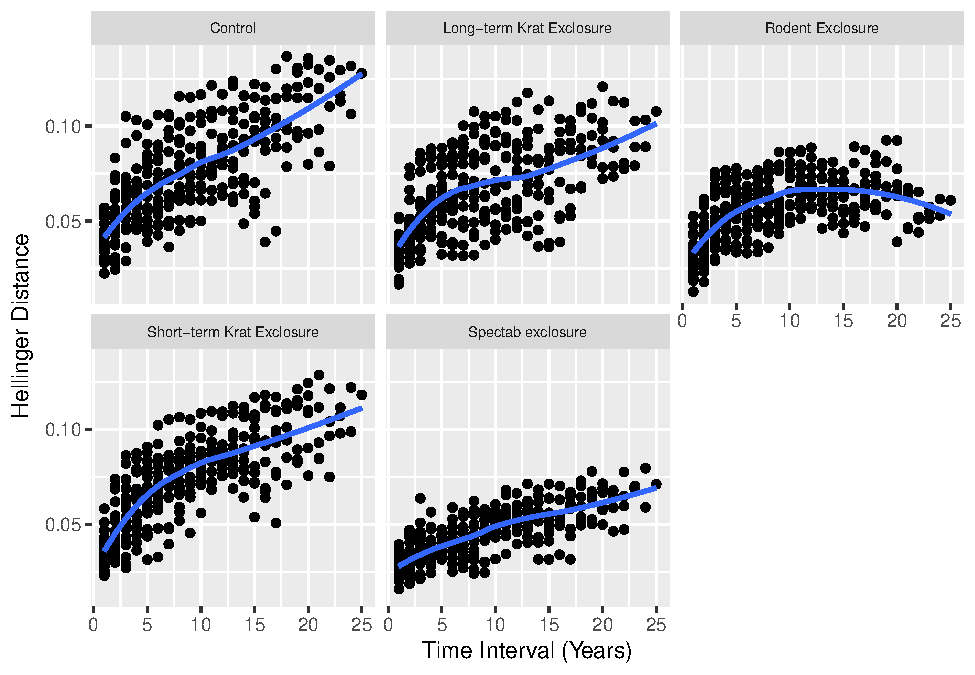
\includegraphics{temporal_assignment_files/figure-latex/unnamed-chunk-8-1.pdf}

\textbf{\emph{Question 7}}:

\begin{enumerate}
\def\labelenumi{\alph{enumi}.}
\tightlist
\item
  What does it mean to calculate a distance metric across varying time
  intervals?
\item
  Interpret the overall results. Develop a hypothesis based on the
  different responses of each treatment.
\end{enumerate}

\begin{quote}
\textbf{\emph{Answer 7a}}: We are calculating how probable similarity
changes over time. In this we can develop hypotheses concerning
community divergence and which can ultimately inform ecological
manamgement and conservation pratices. \textbf{\emph{Answer 7b}}:
Hellinger distances steadily increased through time for all treatments
except for the rodent enclosure, where all rodents were exluded from
entry. Since the rodent enclosure expludes all rodents while the other
treatments include at least on species of rodent, then dispersal
capabilites great influence community divergence over time.
\end{quote}

\subsection{7) STABILITY}\label{stability}

In the R code chunk below, do the following:

\begin{enumerate}
\def\labelenumi{\arabic{enumi}.}
\tightlist
\item
  Using total abundance as your focal variable, calculate stability
  (i.e., 1/CV) and synchrony for each plot type.
\item
  Test for a biodiversity-stability relationship by regressing community
  stability on mean richness.
\item
  Test for a biodiversity-stability relationship by regressing community
  stability on mean inverse Simpson's diversity.
\end{enumerate}

\begin{Shaded}
\begin{Highlighting}[]
\CommentTok{#community stability}
\NormalTok{portal.stab <-}\StringTok{ }\KeywordTok{community_stability}\NormalTok{(}\DataTypeTok{df =} \KeywordTok{as.data.frame}\NormalTok{(portal.species.abunds),}
                                   \DataTypeTok{time.var =} \StringTok{"year"}\NormalTok{,}
                                   \DataTypeTok{abundance.var =} \StringTok{"n"}\NormalTok{,}
                                   \DataTypeTok{replicate.var =} \StringTok{"plot_type"}\NormalTok{)}

\KeywordTok{pander}\NormalTok{(portal.stab)}
\end{Highlighting}
\end{Shaded}

\begin{longtable}[]{@{}cc@{}}
\toprule
\begin{minipage}[b]{0.34\columnwidth}\centering\strut
plot\_type\strut
\end{minipage} & \begin{minipage}[b]{0.14\columnwidth}\centering\strut
stability\strut
\end{minipage}\tabularnewline
\midrule
\endhead
\begin{minipage}[t]{0.34\columnwidth}\centering\strut
Control\strut
\end{minipage} & \begin{minipage}[t]{0.14\columnwidth}\centering\strut
3.044\strut
\end{minipage}\tabularnewline
\begin{minipage}[t]{0.34\columnwidth}\centering\strut
Long-term Krat Exclosure\strut
\end{minipage} & \begin{minipage}[t]{0.14\columnwidth}\centering\strut
1.865\strut
\end{minipage}\tabularnewline
\begin{minipage}[t]{0.34\columnwidth}\centering\strut
Rodent Exclosure\strut
\end{minipage} & \begin{minipage}[t]{0.14\columnwidth}\centering\strut
1.864\strut
\end{minipage}\tabularnewline
\begin{minipage}[t]{0.34\columnwidth}\centering\strut
Short-term Krat Exclosure\strut
\end{minipage} & \begin{minipage}[t]{0.14\columnwidth}\centering\strut
2.462\strut
\end{minipage}\tabularnewline
\begin{minipage}[t]{0.34\columnwidth}\centering\strut
Spectab exclosure\strut
\end{minipage} & \begin{minipage}[t]{0.14\columnwidth}\centering\strut
2.911\strut
\end{minipage}\tabularnewline
\bottomrule
\end{longtable}

\begin{Shaded}
\begin{Highlighting}[]
\CommentTok{#species synchrony}
\NormalTok{portal.loreau <-}\StringTok{ }\KeywordTok{synchrony}\NormalTok{(}\DataTypeTok{df =} \KeywordTok{as.data.frame}\NormalTok{(portal.species.abunds),}
                           \DataTypeTok{time.var =} \StringTok{"year"}\NormalTok{,}
                           \DataTypeTok{species.var =} \StringTok{"taxon"}\NormalTok{,}
                           \DataTypeTok{abundance.var =} \StringTok{"n"}\NormalTok{,}
                           \DataTypeTok{replicate.var =} \StringTok{"plot_type"}\NormalTok{,}
                           \DataTypeTok{metric =} \StringTok{"Loreau"}\NormalTok{)}

\KeywordTok{names}\NormalTok{(portal.loreau)[}\DecValTok{2}\NormalTok{] <-}\StringTok{ "loreau"}

\NormalTok{portal.gross <-}\StringTok{ }\KeywordTok{synchrony}\NormalTok{(}\DataTypeTok{df =} \KeywordTok{as.data.frame}\NormalTok{(portal.species.abunds),}
                          \DataTypeTok{time.var =} \StringTok{"year"}\NormalTok{,}
                          \DataTypeTok{species.var =} \StringTok{"taxon"}\NormalTok{,}
                          \DataTypeTok{abundance.var =} \StringTok{"n"}\NormalTok{,}
                          \DataTypeTok{replicate.var =} \StringTok{"plot_type"}\NormalTok{,}
                          \DataTypeTok{metric =} \StringTok{"Gross"}\NormalTok{)}

\KeywordTok{names}\NormalTok{(portal.gross)[}\DecValTok{2}\NormalTok{] <-}\StringTok{ "gross"}

\KeywordTok{pander}\NormalTok{(}\KeywordTok{full_join}\NormalTok{(portal.loreau, portal.gross))}
\end{Highlighting}
\end{Shaded}

\begin{verbatim}
## Joining, by = "plot_type"
\end{verbatim}

\begin{longtable}[]{@{}ccc@{}}
\toprule
\begin{minipage}[b]{0.33\columnwidth}\centering\strut
plot\_type\strut
\end{minipage} & \begin{minipage}[b]{0.11\columnwidth}\centering\strut
loreau\strut
\end{minipage} & \begin{minipage}[b]{0.11\columnwidth}\centering\strut
gross\strut
\end{minipage}\tabularnewline
\midrule
\endhead
\begin{minipage}[t]{0.33\columnwidth}\centering\strut
Control\strut
\end{minipage} & \begin{minipage}[t]{0.11\columnwidth}\centering\strut
0.1869\strut
\end{minipage} & \begin{minipage}[t]{0.11\columnwidth}\centering\strut
0.1263\strut
\end{minipage}\tabularnewline
\begin{minipage}[t]{0.33\columnwidth}\centering\strut
Long-term Krat Exclosure\strut
\end{minipage} & \begin{minipage}[t]{0.11\columnwidth}\centering\strut
0.1578\strut
\end{minipage} & \begin{minipage}[t]{0.11\columnwidth}\centering\strut
0.07418\strut
\end{minipage}\tabularnewline
\begin{minipage}[t]{0.33\columnwidth}\centering\strut
Rodent Exclosure\strut
\end{minipage} & \begin{minipage}[t]{0.11\columnwidth}\centering\strut
0.187\strut
\end{minipage} & \begin{minipage}[t]{0.11\columnwidth}\centering\strut
0.1423\strut
\end{minipage}\tabularnewline
\begin{minipage}[t]{0.33\columnwidth}\centering\strut
Short-term Krat Exclosure\strut
\end{minipage} & \begin{minipage}[t]{0.11\columnwidth}\centering\strut
0.08773\strut
\end{minipage} & \begin{minipage}[t]{0.11\columnwidth}\centering\strut
0.001546\strut
\end{minipage}\tabularnewline
\begin{minipage}[t]{0.33\columnwidth}\centering\strut
Spectab exclosure\strut
\end{minipage} & \begin{minipage}[t]{0.11\columnwidth}\centering\strut
0.1542\strut
\end{minipage} & \begin{minipage}[t]{0.11\columnwidth}\centering\strut
0.1393\strut
\end{minipage}\tabularnewline
\bottomrule
\end{longtable}

\begin{Shaded}
\begin{Highlighting}[]
\CommentTok{#variance ratio}
\NormalTok{portal.vr <-}\StringTok{ }\KeywordTok{variance_ratio}\NormalTok{(}\DataTypeTok{df =} \KeywordTok{as.data.frame}\NormalTok{(portal.species.abunds),}
                            \DataTypeTok{time.var =} \StringTok{"year"}\NormalTok{, }\DataTypeTok{species.var =} \StringTok{"taxon"}\NormalTok{,}
                            \DataTypeTok{abundance.var =} \StringTok{"n"}\NormalTok{, }\DataTypeTok{replicate.var =} \StringTok{"plot_type"}\NormalTok{,}
                            \DataTypeTok{bootnumber =} \DecValTok{1000}\NormalTok{, }\DataTypeTok{average.replicates =} \NormalTok{T,}
                            \DataTypeTok{level =} \FloatTok{0.95}\NormalTok{)}
\KeywordTok{pander}\NormalTok{(portal.vr)}
\end{Highlighting}
\end{Shaded}

\begin{longtable}[]{@{}cccc@{}}
\toprule
\begin{minipage}[b]{0.12\columnwidth}\centering\strut
lowerCI\strut
\end{minipage} & \begin{minipage}[b]{0.12\columnwidth}\centering\strut
upperCI\strut
\end{minipage} & \begin{minipage}[b]{0.14\columnwidth}\centering\strut
nullmean\strut
\end{minipage} & \begin{minipage}[b]{0.06\columnwidth}\centering\strut
VR\strut
\end{minipage}\tabularnewline
\midrule
\endhead
\begin{minipage}[t]{0.12\columnwidth}\centering\strut
0.6864\strut
\end{minipage} & \begin{minipage}[t]{0.12\columnwidth}\centering\strut
1.393\strut
\end{minipage} & \begin{minipage}[t]{0.14\columnwidth}\centering\strut
1.006\strut
\end{minipage} & \begin{minipage}[t]{0.06\columnwidth}\centering\strut
1.325\strut
\end{minipage}\tabularnewline
\bottomrule
\end{longtable}

\begin{Shaded}
\begin{Highlighting}[]
\CommentTok{#biodiversity-stability}
\NormalTok{portal.mean.rich.plot <-}\StringTok{ }\NormalTok{rich.all %>%}
\StringTok{  }\KeywordTok{group_by}\NormalTok{(plot_id) %>%}
\StringTok{  }\KeywordTok{summarise}\NormalTok{(}\DataTypeTok{mean.rich =} \KeywordTok{mean}\NormalTok{(richness))}

\NormalTok{portal.plot.abunds <-}\StringTok{ }\KeywordTok{as.data.frame}\NormalTok{(}
  \KeywordTok{group_by}\NormalTok{(portal, year, plot_id) %>%}\StringTok{ }\KeywordTok{count}\NormalTok{(taxon))}

\NormalTok{portal.stab.plot <-}\StringTok{ }\KeywordTok{community_stability}\NormalTok{(}\DataTypeTok{df =} \NormalTok{portal.plot.abunds,}
                                        \DataTypeTok{time.var =} \StringTok{"year"}\NormalTok{,}
                                        \DataTypeTok{abundance.var =} \StringTok{"n"}\NormalTok{,}
                                        \DataTypeTok{replicate.var =} \StringTok{"plot_id"}\NormalTok{)}

\NormalTok{portal.div.stab <-}\StringTok{ }\NormalTok{portal.mean.rich.plot %>%}
\StringTok{  }\KeywordTok{inner_join}\NormalTok{(portal.stab.plot)}
\end{Highlighting}
\end{Shaded}

\begin{verbatim}
## Joining, by = "plot_id"
\end{verbatim}

\begin{Shaded}
\begin{Highlighting}[]
\KeywordTok{par}\NormalTok{(}\DataTypeTok{mar =} \KeywordTok{c}\NormalTok{(}\DecValTok{5}\NormalTok{,}\DecValTok{5}\NormalTok{,}\DecValTok{1}\NormalTok{,}\DecValTok{1}\NormalTok{))}

\KeywordTok{plot}\NormalTok{(portal.div.stab$stability ~}\StringTok{ }\NormalTok{portal.div.stab$mean.rich,}
     \DataTypeTok{xlab =} \StringTok{""}\NormalTok{, }\DataTypeTok{ylab =} \StringTok{""}\NormalTok{, }\DataTypeTok{yaxt =} \StringTok{"n"}\NormalTok{, }\DataTypeTok{xaxt =} \StringTok{"n"}\NormalTok{,}
     \DataTypeTok{xlim =} \KeywordTok{c}\NormalTok{(}\DecValTok{2}\NormalTok{,}\DecValTok{10}\NormalTok{), }\DataTypeTok{ylim =} \KeywordTok{c}\NormalTok{(}\DecValTok{1}\NormalTok{,}\DecValTok{4}\NormalTok{))}
\KeywordTok{axis}\NormalTok{(}\DataTypeTok{side =} \DecValTok{1}\NormalTok{, }\DataTypeTok{cex.axis =} \FloatTok{1.2}\NormalTok{, }\DataTypeTok{lwd.ticks =} \DecValTok{2}\NormalTok{, }\DataTypeTok{las =} \DecValTok{1}\NormalTok{)}
\KeywordTok{axis}\NormalTok{(}\DataTypeTok{side =} \DecValTok{2}\NormalTok{, }\DataTypeTok{cex.axis =} \FloatTok{1.2}\NormalTok{, }\DataTypeTok{lwd.ticks =} \DecValTok{2}\NormalTok{, }\DataTypeTok{las =} \DecValTok{1}\NormalTok{)}
\KeywordTok{axis}\NormalTok{(}\DataTypeTok{side =} \DecValTok{3}\NormalTok{, }\DataTypeTok{lwd.ticks =} \DecValTok{2}\NormalTok{, }\DataTypeTok{las =} \DecValTok{1}\NormalTok{, }\DataTypeTok{labels =} \NormalTok{F)}
\KeywordTok{axis}\NormalTok{(}\DataTypeTok{side =} \DecValTok{4}\NormalTok{, }\DataTypeTok{lwd.ticks =} \DecValTok{2}\NormalTok{, }\DataTypeTok{las =} \DecValTok{1}\NormalTok{, }\DataTypeTok{labels =} \NormalTok{F)}
\KeywordTok{box}\NormalTok{(}\DataTypeTok{lwd =} \DecValTok{2}\NormalTok{)}
\KeywordTok{mtext}\NormalTok{(}\StringTok{"Mean Richness"}\NormalTok{, }\DataTypeTok{side =} \DecValTok{1}\NormalTok{, }\DataTypeTok{line =} \DecValTok{3}\NormalTok{, }\DataTypeTok{cex =} \FloatTok{1.5}\NormalTok{)}
\KeywordTok{mtext}\NormalTok{(}\StringTok{"Aggregate Stability"}\NormalTok{, }\DataTypeTok{side =} \DecValTok{2}\NormalTok{, }\DataTypeTok{line =} \FloatTok{3.5}\NormalTok{, }\DataTypeTok{cex =} \FloatTok{1.5}\NormalTok{)}
\KeywordTok{mtext}\NormalTok{(}\KeywordTok{expression}\NormalTok{(}\KeywordTok{paste}\NormalTok{(}\StringTok{"(CV"}\NormalTok{^}\StringTok{"-1"}\NormalTok{,}\StringTok{" Total Abundance)"}\NormalTok{)),}
      \DataTypeTok{side =} \DecValTok{2}\NormalTok{, }\DataTypeTok{line =} \FloatTok{2.25}\NormalTok{, }\DataTypeTok{cex =} \NormalTok{.}\DecValTok{8}\NormalTok{)}

\NormalTok{div.stab.lm <-}\StringTok{ }\KeywordTok{lm}\NormalTok{(portal.div.stab$stability ~}\StringTok{ }\NormalTok{portal.div.stab$mean.rich)}

\KeywordTok{abline}\NormalTok{(div.stab.lm)}

\NormalTok{r2 <-}\StringTok{ }\KeywordTok{bquote}\NormalTok{(}\KeywordTok{italic}\NormalTok{(R)^}\DecValTok{2} \NormalTok{==}\StringTok{ }\NormalTok{.(}\KeywordTok{format}\NormalTok{(}
  \KeywordTok{summary}\NormalTok{(div.stab.lm)$adj.r.square, }\DataTypeTok{digits =} \DecValTok{3}\NormalTok{)))}
\KeywordTok{text}\NormalTok{(}\FloatTok{3.25}\NormalTok{,}\FloatTok{3.75}\NormalTok{, }\DataTypeTok{cex =} \FloatTok{1.5}\NormalTok{, }\DataTypeTok{labels =} \NormalTok{r2)}
\end{Highlighting}
\end{Shaded}

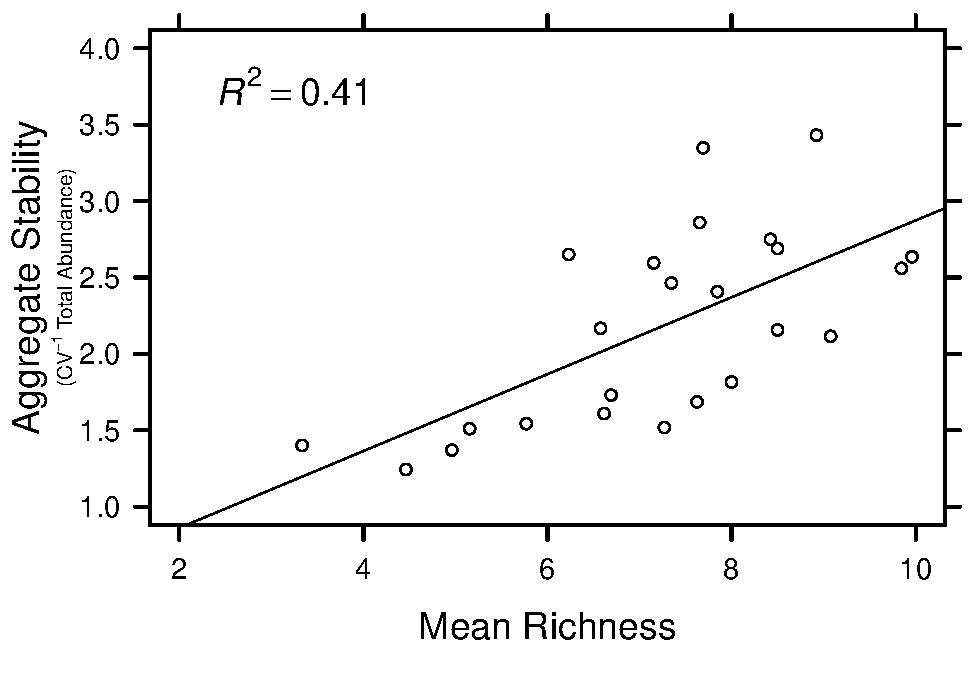
\includegraphics{temporal_assignment_files/figure-latex/unnamed-chunk-9-1.pdf}

\textbf{\emph{Question 8}}:

\begin{enumerate}
\def\labelenumi{\alph{enumi}.}
\tightlist
\item
  Which plot type has the highest stability in total abundance? How is
  stability of total abundance measured with the function you learned?
  How does this measure of stability relate to the coefficient of
  variation?
\item
  In your own words, describe the concept of synchrony
\item
  Interpret the results from the biodiversity-stability relationships
  you analyzed.
\end{enumerate}

\begin{quote}
\textbf{\emph{Answer 8a}}: The control plot has the highest stability
(stability = 3.04). Stability with this function is measured by taking
the reciprical of the standard deviation over the mean of the variable
(in this case abundance). This relates to the coefficient of variation
because this coeffient is simply the standard deviation over the mean of
the variable - so, while a higher coefficient of variation equals higher
variation, a higher stability value equals less variation.
\textbf{\emph{Answer 8b}}: Synchrony in the context of this assignment
is referring to how the community structure of species responds to
varying conditions. For example, if all species across treatments
expreience a reduciton in numbers as a results of a climatical event,
then community structure is synchroneous among treatment groups. If the
same climatic event yeilds decresed numbers of some species and not
others, then community structure would be considered asynchroneous.
\textbf{\emph{Answer 8c}}: Across plot types, richness and stability are
increasing over time however the correlation is only of moderate strngth
(r2 = 0.41).
\end{quote}

\subsection{SYNTHESIS}\label{synthesis}

Compare and contrast the core concepts from temporal and spatial
diversity (e.g., autocorrelation, scale, variability, etc.). Identify a
few of the major challenges associated with studying biodiversity
through time and across space.

\begin{quote}
\textbf{\emph{Answer}}: Autocorrelation between temporal and spatial
scales are similar in that they are looking for internal correlative
patters, however they are caluculated differently. Spatially is
essentially less complex because it is looking at a single point in time
and does not have to account for lag time effects as needs to be
considered with temporal autocorrelation. Scale is also similar between
evaluating spatial and temporal data - however, they are referring to
two particularly different things. In spatial analyses scale is
referring to the size of the study area - for example, how many square
kilometers are needed to caluculate diversity of grasses in central
park? In temoral analyses, lenth of time is the scale - using the same
example, how many years should diversity be measured to understand
succession of grasses since the contruciton of Central Park?
Variability, like scale, is a similar concept within spatial and
temporal diversity but it is estimated in different ways depending on
your study. In spatial ecology variabiliy is measuring a single instance
while in temporal ecology isis measuring change in variability over
time. That said, you do need to look at variability of the spaital scope
of your temporal analyses in order to look at how that variability
changed over time. Stability is a concept that is only useful for
temporal/spatiotemporal studies because it innately implies change over
time. However, turnover can work for both space and time independently -
you can look at turnover through years or between sites at a given point
in time.
\end{quote}

\begin{quote}
Studying biodiversity through space and time can be challenging,
especially if you want to generate future forcasts. This is primarily
true because it is very difficult to account for all of the
ever-changing variables that might be influencing biodiversity in any
given area. This becomes exceptionally complicated if you consider
humana activiy. For exmaple, if you are attempting to forcast how
diversity and age class of trees in a park will look in the future, how
do you account for changing managment practices of the city in which the
park is located? Can you adequately predict if funding will even allow
for management? Furthermore, identifying the appropriate scope of a
project is difficult as well - how much/little space and time is
necessary to adequatly measure the phenomonon you are attempting to
describe? Is four years enough time to measure succession rates after a
forest fire? 10 years? How much of the affected area is enough to sample
in order to get a representative subset of the entire ecoregion?
\end{quote}


\end{document}
